\section{\texorpdfstring{\LFCR}\,: Design and Insights}
\label{sec:CFL}

When solving a CFL-reachability problem with a CFL, the CFL and its underlying graph
structure are always inter-connected and carefully designed together. To break their cyclic
dependencies, we first describe how to represent a program with a new \pag representation 
to facilitate on-the-fly call graph construction
(\Cref{subsec:newPAG}). We then
formalize \LFCR by explaining how we address the three challenges
(\challenge{1} -- \challenge{3}) and providing some insights
in understanding its design (\Cref{subsec:newCFLs}).
% In \Cref{subsec:discussion}, we discuss 
% some topics related to our new formulation. 


\subsection{Pointer Assignment Graph} 
\label{subsec:newPAG}

%Like previous pointer analyses formulated in CFL-reachability \cite{sridharan2005demand, sridharan2006refinement, lu2019precision, lu2021eagle}, our formulation also operates on a graph representation of the program, known as \textit{pointer assignment graph} (\pag). 

For a program, we use the rules given in 
\Cref{fig:newcflpag} to build a \pag representation for \LFCR. We first introduce
these rules briefly by highlighting their differences  from those adopted by \manuLFC
(\Cref{fig:manucflpag}) 
for building an \manuLFC-oriented PAG representation. We then illustrate these rules with an example.
Note that one is expected to develop a reasonably good understanding of this new PAG representation before 
examining the three CFLs used for defining
\LFCR later.
%, whose nodes 
%represent variables and heap objects, and whose edges represent the value flows through 
%assignments. 

As in the case of \manuLFC (\Cref{fig:manucflpag}), the inverse of a PAG edge
is not given
explicitly. For each \pag edge 
$x\xrightarrow[c]{\ell}y$, its inverse edge is defined as  
$y\xrightarrow[\overline{c}]{\overline{\ell}}x$ as in \manuLFC exactly  (\Cref{subsubsec:CFLReachability}),
except that 
a below-edge label can also be $\hat{\boxed{c}}$ or $\check{\boxed{c}}$
(in addition to $\hat{{c}}$ and $\check{{c}}$), in which case,
$\overline{\hat{\boxed{c}}}=\check{\boxed{c}}$ and $\overline{\check{\boxed{c}}}=\hat{\boxed{c}}$, where $c$ identifies a  callsite.
To trigger dynamic dispatch at a callsite $c$, an edge with a boxed below-edge label also represents conceptually 
a new kind of inter-procedural value-flow entering into (marked by 
$\hat{\boxed{c}}$)
or exiting from (marked by 
$\check{\boxed{c}}$) from a method invoked at  $c$. Such boxed below-edge labels are
introduced for addressing \challenge{3} only and their significance will become clear
in \Cref{subsubsec:newLR}.

%implying that the concepts
%of entry and exit contexts  for inter-context
%value-flow edges are swapped if they are
%  traversed inversely. 



 

%The rules for adding $\mathtt{y} 
%\xrightarrow{\assign} \mathtt{x}$, $\mathtt{y} \xrightarrow{\loadfield{f}} \mathtt{x}$, and 
%$\mathtt{y} \xrightarrow{\storefield{f}} \mathtt{x}$,
%which are also used in earlier work
%\cite{sridharan2005demand, sridharan2006refinement, lu2019precision, lu2021eagle}, 

% $\tau$ is a placeholder used in $L_C$ for context recovery, which will be introduced shortly.  


\begin{figure}[t]
\begin{center}
% \vspace*{-1ex}
% \begin{adjustbox}{width=1\linewidth}
\begin{tabular}{c}
			\ruledef{
				 \mathtt{x = \mathsf{\mathbf{new}} ~ T} ~ { \mathtt{//~O}}
			}{
				O \xrightarrow{\new[\texttt{T}]} \mathtt{x} 
				% \rulespace
				% \mathtt{o} \xrightarrow[\tau]{\typefound[t]} \mathtt{o}
			}
		 \rulename{C-New} 
		 \quad
			\ruledef{
			    \mathtt{x = y} 
			}{
				\mathtt{y} \xrightarrow{\assign} \mathtt{x}
			}
			\rulename{C-Assign}
			 \\[6ex]
	 		\ruledef{
            			    \mathtt{x = y.f} 
            			}{
            				\mathtt{y} \xrightarrow{\load[\texttt{f}]} \mathtt{x}
            			}
        	 \rulename{C-Load}
        	 \quad
			\ruledef{
			    \mathtt{x.f = y} 
			}{
				\mathtt{y} \xrightarrow{\store[\texttt{f}]} \mathtt{x} 
			}
			 \rulename{C-Store}
             \\[6ex]
        %      \ruledef{
        %     			}{
        %     				% 			\mathtt{this}^{m} \xrightarrow{\load[i]} \mathtt{p_i^m}
        %     							\mathtt{m} \xrightarrow{\assign} \mathtt{this^m}
        %     			}
        
        % 	 \rulename{This}
        %      \quad
   
             			\ruledef{
			   \mathtt{x = } ~ \mathtt{m}(a_1, \dots, a_n) ~ \mathtt{//~ c} 
			}{
			\rulespace \forall \ i \in [1, n]: a_i \xrightarrow[\hat{c} ]{\assign} p_i^{\mathtt{m}}
			\rulespace \mathtt{ret}^\mathtt{m} \xrightarrow[\check{c}]{\assign} \mathtt{x}
% 			\rulespace a_0 \xrightarrow[\hat{\boxed{c}}]{\assign} a_0 \\
% 			\rulespace {a_0 \xrightarrow[\check{\boxed{c}}]{\assign} a_0\#\texttt{c} }
%             \rulespace a_0\#\texttt{c} \xrightarrow[\hat{c} ]{\indispatch[t]} \mathtt{this}^{m'}
			}
			\rulename{C-SCall}
			\\[7ex]
% 			\ruledef{
% 			   \mathtt{x = } ~ \mathtt{r}.\mathtt{m}(a_1,..., a_n) ~ \mathtt{//~ c} 
% 			 %  \rulespace o \in \cipointsto{a_0} 
% 			   \rulespace t <: \decltypeof(\mathtt{r})
% 			   \rulespace m' = \lookup(\texttt{m}, t) 
% 			}{
% 			\rulespace \forall \ i \in [1, n]: a_i \xrightarrow[\hat{\boxed{c}} ]{\store[i]} \mathtt{r}
% 			\rulespace \mathtt{r} \xrightarrow[\check{\boxed{c}}]{\load[\ret]} \mathtt{x}
% 			\rulespace \mathtt{r} \xrightarrow[\hat{\boxed{c}}]{\assign} \mathtt{r} \\
% 			\rulespace {\mathtt{r} \xrightarrow[\check{\boxed{c}}]{\assign} \mathtt{r}\#\texttt{c} }
%             \rulespace \mathtt{r}\#\texttt{c} \xrightarrow[\hat{c} ]{\indispatch[t]} \mathtt{this}^{m'}
% 			}
% 			\rulename{C-VCall}
% 			\\[5ex]
			\ruledef{
			   \mathtt{x = } ~ \mathtt{r}.\mathtt{m}(a_1, \dots, a_n) ~ \mathtt{//~ c} 
			 %  \rulespace o \in \cipointsto{a_0} 
			   \rulespace \texttt{t} <: \decltypeof(\mathtt{r})
			   \rulespace \mathtt{m'} = \lookup(\texttt{m}, \texttt{t}) 
			}{
			\rulespace \forall \ i \in [1, n]: a_i \xrightarrow[\hat{\boxed{c}} ]{\store[i]} \mathtt{r}
			\rulespace \mathtt{r} \xrightarrow[\check{\boxed{c}}]{\load[\ret]} \mathtt{x}
			\rulespace \mathtt{r} \xrightarrow{\assign} \mathtt{r}\#\texttt{c} \\
			\rulespace {\mathtt{r} \xrightarrow[\check{\boxed{c}}]{\assign} \mathtt{r}\#\texttt{c} }
            \rulespace \mathtt{r}\#\texttt{c} \xrightarrow[\hat{c} ]{\indispatch[\texttt{t}]} \mathtt{this}^{\mathtt{m'}}
			}
			\rulename{C-VCall}
			\\[6ex]
			\\
         	\ruledef{
            	        \mathtt{M} ~ \text{is an instance method} \rulespace
            	        p_i^\mathtt{M} ~ \text{is its }i\text{th parameter }
            			}{
            							\mathtt{this}^{\mathtt{M}} \xrightarrow{\load[i]} p_i^\mathtt{M}
            				% 			\mathtt{m} \xrightarrow{\load[i]} \mathtt{p_i^m}
            			}
        	 \rulename{C-Param}
        %	 \\[5ex]
         	 \quad
			\ruledef{
			    \mathtt{M} ~ \text{is an instance method}
			}{
				\mathtt{ret}^{\mathtt{M}}  \xrightarrow{\store[\ret]} \mathtt{this}^{\mathtt{M}}
				% \mathtt{ret}^{\mathtt{m}}  \xrightarrow{\store[\texttt{ret}]} \texttt{m}
			}
			 \rulename{C-Ret}
  %           \\[5ex]
             
%			\ruledef{
%			    a  \xrightarrow[Y]{X} b
%			}{
%				b  \xrightarrow[\overline{Y}]{\overline{X}} a
%			}
%			 \rulename{Inverse}
		\end{tabular}
% 	\end{adjustbox}
	\end{center}
%	\vspace*{-2ex}
	\caption{Rules for building the PAG required by \LFCR.
%	(where the inverses of 	all the edges are omitted).}
	\label{fig:newcflpag}}
%		\vspace*{-1.5ex}
\end{figure}

Our PAG representation (for supporting \LFCR) differs from that for supporting
\manuLFC
(\Cref{fig:manucflpag}) mainly in  how virtual callsites are handled. Therefore,
\rulename{C-Assign}, \rulename{C-Load}, and \rulename{C-Store} 
are identical to \rulename{P-Assign}, \rulename{P-Load}, and \rulename{P-Store},
 respectively. In addition, \rulename{C-SCall}, which behaves also identically as \rulename{P-SCall}, handles parameter passing at a static callsite $c$  simply as assignments
 in terms of 
 inter-procedural \assign edges, with its entry (exit) context being 
 $\hat{c}$ ($\check{c}$).
 



\rulename{C-New},
\rulename{C-VCall},
\rulename{C-Param}, and
\rulename{C-Ret} build the PAG edges together to enable \LFCR to perform its own on-the-fly call graph construction at virtual callsites (for addressing \challenge{1} and \challenge{2}).
In \rulename{C-New} (unlike \rulename{P-New} in \Cref{fig:manucflpag}), $O \xrightarrow{\!\!\new[\texttt{T}]\!\!} \mathtt{x}$ encodes  explicitly the dynamic
 type \texttt{T} of $O$  in order to support dynamic dispatch on~$O$ while
 also enabling $O$ to be passed as a receiver object to a method (dispatched
 on $O$)
 without the precision loss discussed using the code in 
 \Cref{fig:recvobj}.

Given an instance method $\mathtt{M}$
(with $\texttt{this}^\mathtt{M}$ denoting its \texttt{this} variable),
its  $i$-th  (non-$\texttt{this}$) parameter $p_{i}^{\mathtt{M}}$  (where $i$ starts from 1)
is modeled as a
 special field of  $\texttt{this}^\mathtt{M}$ (identified by   offset $i$) and
its return variable $\mathtt{ret}^\mathtt{M}$ also  as a
 special field of  $\texttt{this}^\mathtt{M}$ (identified by  offset 0).
%(e.g., the $i$-th parameter has an offset of $i$ and the return variable has an offset of 0 which is represented by \texttt{ret}).  
Thus, we can initialize $p_{i}^{\mathtt{M}}$  with a load
 $\mathtt{this}^{\mathtt{M}} \xrightarrow{\load[i]} p_{i}^{\mathtt{M}}$
 %, i.e., $\mathtt{p}_{i}^{M}=\mathtt{this}^M.i$
 (\rulename{C-Param}) 
 and $\mathtt{this}^\mathtt{M}.\ret$ with a store
 $\mathtt{ret}^\mathtt{M}  \xrightarrow{\storefield{\ret}} \mathtt{this}^{\mathtt{M}}$
 %, i.e.,  $\mathtt{this}^M.0 = \mathtt{ret}^{M}$
 (\rulename{C-Ret}).
 

 
 
\rulename{C-VCall}, which is the most complex rule, differs fundamentally from \rulename{P-VCall} (\Cref{fig:manucflpag}) in
handling
a virtual callsite 
``$\mathtt{x = } ~ \mathtt{r}.\mathtt{m}(a_1, \dots, a_n) ~ \mathtt{//~ c}$''. For
convenience,
we make use of $\mathtt{r}\#\texttt{c}$ (a temporary) to identify uniquely this particular
occurrence of
 $\mathtt{r}$ at this callsite. When building the PAG, we over-approximate the
set of target methods invoked at each callsite  (and consequently, the call graph for the
program) by using class hierarchy analysis
(CHA) \cite{dean1995optimization} (due to $\texttt{t} <: \decltypeof(\mathtt{r})$ and
$ \mathtt{m'} = \lookup(\texttt{m}, \texttt{t}) $). It is crucial to highlight
that \hl{(1) CHA relies solely on the type information of a program and has the ability to construct an initial call graph in a linear manner; and  (2)} \LFCR will perform its on-the-fly call graph construction
over such an over-approximated PAG with spurious call targets being 
filtered out (as discussed at the end of 
\Cref{subsec:newCFLs}). To pass a 
non-receiver  argument  
$a_i$ ($1\leqslant i \leqslant n)$ to
the corresponding  parameter $p_i^{\mathtt{m'}}$ 
of a target method, $\mathtt{m'}$, we make use of a  store
$ a_i \xrightarrow[\hat{\boxed{c}}]{\storefield{$i$}} \mathtt{r}$ introduced in this rule 
 and  a matching load
 $\mathtt{this}^{\texttt{m}'} \xrightarrow{\load[i]} p_{i}^{\texttt{m}'}$
 %, i.e., $\mathtt{p}_{i}^{M}=\mathtt{this}^M.i$
 (\rulename{C-Param}).
 By performing CFL-reachability
under \LFCR, 
traversing such an edge will trigger a search
for the dynamic type of
every receiver object pointed to by $\mathtt{r}$ (marked by
$\hat{\boxed{c}}$). Encountering 
$\mathtt{r} \xrightarrow[\check{\boxed{c}}]{\assign} 
\mathtt{r}\#\texttt{c} \xrightarrow[\hat{c}]{\indispatch[\texttt{t}]} \texttt{this}^{\mathtt{m'}} 
$
(introduced in this rule) later signifies that one such a dynamic type \texttt{t} has been found (marked by 
$\check{\boxed{c}}$) so that $\mathtt{m'}$, where $\mathtt{m'} = \lookup(\texttt{m}, \texttt{t})$,
  can be dispatched with $\hat{c}$ as its entry context (as desired), where $c$ is recovered from $\boxed{c}$. By definition, a \reg{dispatch} edge  also serves as an
  \assign edge as well.
  As for the receiver variable $\mathtt{r}$, we 
use  $\mathtt{r} \xrightarrow{\assign} \mathtt{r}\#c$ (without a need for relating
\texttt{r} to 
itself).
Finally, we assign $\mathtt{ret}^{\mathtt{m'}}$ (saved earlier in $\texttt{this}^\texttt{m}.0$)  (\rulename{C-Ret}) 
to \texttt{x} via a load
 $a_0 \xrightarrow[\check{\boxed{c}}]{\loadfield{\ret}} \mathtt{x}$ (introduced in this rule),
 where $\check{\boxed{c}}$ signifies the end of dynamic dispatch on $\mathtt{r}$ on exit
 from  callsite~$c$.

  \begin{figure*}
\centering
\resizebox{0.635\width}{0.69\height}{
\begin{tikzpicture}
    \draw [draw=black!5, fill=black!5] (5.1,1.7) rectangle (11.6,0.8); % A::foo
    \draw [draw=black!5, fill=black!5] (5.1,0.5,0) rectangle (9.6,-0.3); % B::foo
    \draw [draw=black!5, fill=black!5] (5.1,-0.6,0) rectangle (9.6,-1.5);  % C::foo
    \draw [draw=black!5, fill=black!5] (-10.5,1.7,0) rectangle (-3.5,0.9); % main
    \draw [draw=black!5, fill=black!5] (-10.5,-1.5,0) rectangle (-3.5,-.8); % main
    \draw [draw=black!5, fill=black!5] (-10.5,1.5,0) rectangle (-7.5,-1.3); % main
    \draw [draw=black!5, fill=black!5] (-6.5,0.6,0) rectangle (2.5,-0.6); % bar
    \node(x) {\texttt{x}};
    \node(d)[left of =x, xshift=0.5cm] {\texttt{d}};
    \node(D)[left of=d, xshift=1cm, yshift=.0cm] {\texttt{D1}};
    \node(o)[left of=D, xshift=1.5cm] {\texttt{o}};
    \node(o1)[above left of=o, yshift=-1.2cm] {\texttt{o1}};
    \node(O1)[left of=o1, xshift=1cm] {\texttt{O1}};
    \node(o2)[below left of=o, yshift=1.1cm] {\texttt{o2}};
    \node(O2)[left of=o2, xshift=1cm] {\texttt{O2}};
    \node(xc)[right of=x, xshift=-1cm] {\texttt{x\#c3}};
    \node(a)[above left of=x,yshift=-1cm,xshift=-2cm] {\texttt{a}};
    \node(A)[left of=a, xshift=1cm] {\texttt{A1}};
    \node(b)[below left of=x, yshift=.8cm, xshift=-2cm] {\texttt{b}};
    \node(B)[left of=b, xshift=1cm] {\texttt{B1}};
    \node(thisA)[above right of=xc,xshift=2cm,yshift=-1cm] {$\texttt{this}^\texttt{A:foo()}$};
    \node(p)[right of=thisA]{\texttt{p}};
    \node(v)[right of=p,xshift=-1cm]{\texttt{v}};
    \node(thisB)[right of=xc, yshift=0cm, xshift=1.2cm] {$\texttt{this}^\texttt{B:foo()}$};
    \node(q)[right of=thisB] {\texttt{q}};
    \node(thisC)[below right of=xc, xshift=2cm,yshift=1cm] {$\texttt{this}^\texttt{C:foo()}$};
    \node(r)[right of=thisC]{\texttt{r}};
    
    \path[-stealth]
    (O1) edge[sloped] node{$\new[\texttt{O}]$} (o1)
    (O2) edge[sloped] node{$\new[\texttt{O}]$} (o2)
    
    (A) edge[sloped] node{$\new[\texttt{A}]$} (a)
    (B) edge[sloped] node{$\new[\texttt{B}]$} (b)
    
    (D) edge[sloped, above] node{$\new[\texttt{D}]$} (d)
    
    (a) edge[sloped,bend left=25] node{\assign} (x)
    (a) edge[sloped,bend left=25,below] node{$\hat{\mathtt{c1}}$} (x)
    (o1) edge[sloped,bend left=10] node{\assign} (o)
    (o1) edge[sloped,bend left=10,below] node{$\hat{\mathtt{c1}}$} (o)
    
    (b) edge[sloped,bend right=25] node{\assign} (x)
    (b) edge[sloped,bend right=25,below] node{$\hat{\mathtt{c2}}$} (x)
    (o2) edge[sloped,bend right=10] node{\assign} (o)
    (o2) edge[sloped,bend right=10,below] node{$\hat{\mathtt{c2}}$} (o)
    
    (o) edge[sloped, bend right=40] node{$\store[\texttt{f}]$} (d)
    
    (d) edge[sloped,bend left=0] node{$\store[1]$} (x)
    (d) edge[sloped,bend left=0,below] node{$\hat{\boxed{\mathtt{c3}}}$} (x)
    
    (x) edge[sloped,bend right=30] node{$\assign$} ([shift={(-.1,-.2)}]xc)
    (x) edge[sloped,bend right=30,below] node {$\check{\boxed{\mathtt{c3}}}$} ([shift={(-.1,-.2)}]xc)
%    (x) edge[in=60,out=120,loop,looseness=20] node{$\assign$} (x)
%    (x) edge[in=60,out=120,loop,looseness=20,below] node{$\hat{\boxed{\mathtt{c3}}}$} (x)
    (x) edge[sloped,bend left=30] node{$\assign$} ([shift={(-.1,.2)}]xc)
    
    (xc) edge[sloped,bend left=20] node{$\indispatch[\texttt{A}]$} (thisA)
    (xc) edge[sloped,bend left=20,below] node{$\hat{\mathtt{c3}}$} (thisA)
    (thisA) edge[sloped] node{$\load[1]$} (p)
    (p) edge[sloped] node{$\load[\texttt{f}]$} (v)
    
    (xc) edge[sloped] node{$\indispatch[\texttt{B}]$} (thisB)
    (xc) edge[sloped, below] node{$\hat{\mathtt{c3}}$} (thisB)
    (thisB) edge[sloped] node{$\load[1]$} (q)
    
    (xc) edge[sloped,bend right=20] node{$\indispatch[\texttt{C}]$} (thisC)
    (xc) edge[sloped,bend right=20,below] node{$\hat{\mathtt{c3}}$} (thisC)
    (thisC) edge[sloped] node{$\load[1]$} (r)
    ;
\end{tikzpicture}
}
% \vspace*{-3.5ex}
\caption{The PAG for \LFCR constructed for the program given in \Cref{fig:motivatingExample}.}
\label{fig:pag1}
%\vspace*{-1ex}
\end{figure*}
 
\begin{comment}
We  connect every non-receiver-variable argument  
$a_i$ ($1\leqslant i \leqslant r)$ (under  $\hat{c}$) with
its corresponding parameter $p_i^{m'}$ 
of a method, $m'$,
via  $a_0$ (by CFL-reachability) iff $m'$ is
dispatchable on a receiver object pointed to by $a_0$. 

To relate $a_i$ ($1\leqslant i \leqslant r$) with $a_0$ under 
$\hat{c}$, we will first traverse across a \store edge,
$a_i \xrightarrow[\hat{\boxed{c}}]{\storefield{$i$}} a_0$, i.e., $a_0.i=a_i$ (with the
offset 
$i$ being treated as a special field of $a_0$). We then look for the receiver objects
pointed to by $a_0$. For each receiver object $o$ whose dynamic type is $t$, we will
traverse a path

This is achieved by establishing a path 
 $
 a_i \xrightarrow[\hat{\boxed{c}}]{\storefield{$i$}}a_0 \cdots \xrightarrow{\inew[t]}  \mathtt{o} \xrightarrow{\new[t]} \cdots
a_0 \xrightarrow[\check{\boxed{c}}]{\assign} 
a_0\#\texttt{c} \xrightarrow[\hat{c}]{\indispatch[t]} \texttt{this}^{m'}
\xrightarrow{\loadfield{i}} \mathtt{p}_{i}^{M}
$, such that (1) $a_0$ points to $o$ with its dynamic type being $t$,
(2)
 $\hat{\boxed{c}}$ and $\check{\boxed{c}}$ mark the beginning and end of the CFL-reachability
 traversal for finding the dynamic type $t$,
 (3) $m'$  is dispatched under $\hat{c}$, where $m' = \lookup(\texttt{m}, t)$, and (4) 
 $a_0$ is passed to $p_i^{m'}$ via $a_0.i=a_i$ and $p_i^{m'} = \mathtt{this}.i^{m'}$.

\end{comment}
 




% Note that $\check{\boxed{c}};\hat{c}$ represents two contiguous stack symbols of $L_C$ and must be processed in turn in one transaction. \Cref{subsec:discussion} will discuss how to transform such edges as normal edges with at most one stack symbol as usual.


% Let $L$ be a CFL over $\Sigma$, which is an alphabet drawn  from
% all the edge labels in $G$.
% Each path $p$ in $G$ has a label $L(p)$ in $\Sigma^*$
% formed by concatenating
% in order the labels of the edges in $p$. A node $v$ is \emph{$L$-reachable} from a
% node $u$ if there exists a path $p$ from $u$ to $v$ in $G$, called an \emph{$L$-path}, such
% that $L(p)\in L$.
% To reason about CFL-reachability, we need to traverse the
% edges in $G$ both forwards and backwards.


% For a path $p$ in $G$ such that
% its label is $L(p)=\ell_1,\cdots,\ell_r$ in $L$, the inverse of $p$, i.e.,
% $\overline{p}$ has the label
% $L(\overline{p})=\overline{\ell_r},\cdots,
% \overline{\ell_1}$.



\Cref{fig:pag1} depicts the PAG  used by \LFCR for our motivating example given in ~\Cref{fig:motivatingExample}. As shown, this PAG
(referred to below), which is designed to enable \LFCR to perform
its own built-in on-the-fly call graph construction,
is fundamentally different from the PAG (\Cref{fig:pag2}) used by \manuLFC.

%We will use this PAG for illustration purposes later.



\begin{comment}
For all heap objects, \texttt{A}, \texttt{B}, \texttt{O1}, \texttt{O2} and \texttt{D}, 
a \new edge is added with their respective types being recorded. For static calls, arguments are connected with their corresponding parameters:
$\texttt{a} \xrightarrow[\check{\texttt{c1}}]{\assign} \texttt{x}$,
$\texttt{b} \xrightarrow[\check{\texttt{c2}}]{\assign} \texttt{x}$,
$\texttt{o1} \xrightarrow[\check{\texttt{c1}}]{\assign} \texttt{o}$, and
$\texttt{o2} \xrightarrow[\check{\texttt{c2}}]{\assign} \texttt{o}$.
For the instance calls, all arguments are connected with their corresponding receivers:
$\texttt{x}\xrightarrow[\hat{\boxed{\texttt{c3}}}]{\assign}\texttt{x}$,
$\texttt{d}\xrightarrow[\hat{\boxed{\texttt{c3}}}]{\store[1]}\texttt{x}$, and receivers are connected with their representations at the callsites: 
$\texttt{x} \xrightarrow[\check{\boxed{\mathtt{c3}}}]{\assign} \mathtt{x\#c3}$.
Correspondingly, 
parameters are loaded inside their methods:
% $\texttt{this}^\texttt{A:foo()}\xrightarrow{\load[0]}\texttt{this}^\texttt{A:foo()}$,
$\texttt{this}^\texttt{A:foo()} \xrightarrow{\load[1]}p$,
% $\texttt{this}^\texttt{B:foo()}\xrightarrow{\load[0]}\texttt{this}^\texttt{B:foo()}$,
$\texttt{this}^\texttt{B:foo()}\xrightarrow{\load[1]}q$,
% $\texttt{this}^\texttt{C:foo()}\xrightarrow{\load[0]}\texttt{this}^\texttt{C:foo()}$, 
and
$\texttt{this}^\texttt{C:foo()}\xrightarrow{\load[1]}r$. Finally, dispatch edges are added
between representation of receivers and ``this'' parameter according to different dispatching targets:
$\texttt{x\#c3}\xrightarrow[\hat{\texttt{c3}}]{\indispatch[\mathtt{A}]}\texttt{this}^\texttt{A:foo()}$,
$\texttt{x\#c3}\xrightarrow[ \hat{\texttt{c3}}]{\indispatch[\mathtt{B}]}\texttt{this}^\texttt{B:foo()}$ and
$\texttt{x\#c3}\xrightarrow[\hat{\texttt{c3}}]{\indispatch[\mathtt{C}]}\texttt{this}^\texttt{C:foo()}$.
($\texttt{x\#c3}\xrightarrow[\hat{\texttt{c3}}]{\indispatch[\mathtt{C}]}\texttt{this}^\texttt{C:foo()}$ 
would not be established if PAG is built relying on a context-insensitive pointer analysis.)
\end{comment}


\subsection{\texorpdfstring{\LFCR}{}}
\label{subsec:newCFLs}

%In this section, we present a new CFL-reachability formulation for fully  
%callsite-sensitive and field-sensitive pointer analysis that supports 
%dynamic virtual call dispatching. 

We  express
\LFCR   as the intersection of three CFLs, \capLFCR, 
with each  specifying a
different aspect of \kcs{k}. 
In  \Cref{subsubsec:newLF}, we  introduce \LF,
which describes  field accesses and
dynamic dispatch, for addressing
\challenge{1} and \challenge{2} (\Cref{subsubsec:newLF}). 
\LC, which is given in \Cref{eqn:callsiteLC},  
 enforces callsite-sensitivity by using the
 below-edge terminals $\hat{c}$ and
$\check{c}$
 in the standard manner.
In  \Cref{subsubsec:newLR},
we  introduce \LR (defined over the terminals $\hat{c}$ and
$\check{c}$, $\hat{\boxed{c}}$, and
$\check{\boxed{c}}$), to
  ensure  that parameter passing happens correctly 
in the presence of on-the-fly call
graph construction, for addressing
 \challenge{3}. We shall restrict our discussions to parameter passing  as method
 returns are handled in the same way. 
 When introducing the grammars for \LF and \LR below,
all the double-label \pag edges in a given \pag
are handled in the same way as we have done to \manuLF and \manuLC,
as described in
 \Cref{subsubsec:CFLReachability}.

We shall speak of an \LFC-path as we do for \manuLFC-path (\Cref{subsubsec:manuLFC}). Similarly, we shall
also speak of an \LFCR-path $p$ with the understanding that  
$\LF(p)\in \LF$, 
$\LC(p)\in \LC$, and
$\LR(p)\in \LR$. 

\hl{
To incorporate call graph construction into a CFL-reachability formulation, as defined below, it is necessary to ensure its soundness by guaranteeing that it provides an over-approximation of the set of target methods resolved at a callsite. This means that the constructed call graph should include all possible target methods that could be called at a given callsite. Furthermore, precision is maintained by excluding any spurious target methods from the resolution, ensuring that only relevant and accurate target methods are considered. 
}

\begin{defn}[Soundness and Precision]
\label{def:sound-prec}
Let $L$ be a CFL-reachability formulation that differs from \manuLFC only in
how they handle parameter passing at
virtual callsites, where $L$ itself specifies dynamic method dispatch at virtual callsites
(i.e., performs its 
own built-in
call graph construction) and \manuLFC relies on a separate algorithm $\mathcal{A}$ (by, e.g., calling
\manuLFC recursively to find the receiver objects of virtual callsites under some given contexts)  for performing call graph construction on the fly (Sec.~\ref{sec:LFC+fly}).
Consider a virtual callsite
``$\mathtt{r}.\mathtt{m}(a_1, \dots, a_n); ~ //~ \mathtt{c}$'', where parameter passing  takes place under a given context \CC. Let $T$ be the set of
target methods found by $\mathcal{A}$
at this callsite under $\CC$ (i.e., found also by \manuLFC if a points-to query is issued
for \texttt{r}
for this callsite under $\CC$ separately)
so that \manuLFC can
perform parameter passing for these methods. Then
$L$ is  \emph{sound} if it  enables parameter passing  to be performed
under $\CC$ for at least all
the target methods in $T$ and $L$ is \emph{precise} (in addition to being
sound) if it  enables parameter passing under $\CC$ for exactly the
same target methods in $T$. 
\end{defn}
We shall see that \LFC is  sound (but imprecise) but \LFCR is  precise 
(and obviously  sound).

Let us
consider parameter passing for an argument at a virtual call site
``$\mathtt{r}.\mathtt{m}(a_1, \dots, a_n); ~ // \mathtt{c}$'' 
under a given context $\CC$. In the special case when
 the argument is the receiver variable $\mathtt{r}$, which points  directly to a set of receiver objects, we only need to address \challenge{1} by passing a receiver object
to a target method $m'$ when $m'$ can be dispatched on the receiver object.
If the argument is $a_i$,
the basic idea in addressing
 \challenge{2} and \challenge{3} (facilitated by the PAG designed 
 according to
 the rules given in 
 \Cref{fig:newcflpag})
is to first store  $a_i$  into $\mathtt{r}.i$ (at its special field $i$), then discover the dynamic type $\texttt{t}$ of every receiver object
pointed to by $\mathtt{r}$ under $\CC$ and propagate $\texttt{t}$ to the callsite \texttt{c} where $ \mathtt{m'} = \lookup(\texttt{m}, \texttt{t})$,
and finally, assign
$\texttt{this}^{\mathtt{m}'}.i$ to $p_i^{\mathtt{m}'}$ for this callsite under
still the same given context \CC. As discussed earlier, method returns are
handled similarly.

\begin{comment}
Let \manuLFCDD be the demand-driven formulation of \manuLFC for solving \kcs{k}
by using a
separate algorithm for on-the-fly construction under the assumption that
it can handle parameter passing for receiver variables correctly (without
suffering from the precision loss discussed in Sec.~\ref{sec:LFC+fly}). 
\LFCR is designed to solve \kcs{k}  with CFL-reachability fully  by computing the same points-to information as \manuLFCDD.
Consider our motivating example in \Cref{fig:motivatingExample}.
As discussed in Sec.~\ref{sec:LFC+fly}, \manuLFCDD will assert that \texttt{v} 
points to
 \commentfont{O1} only due to the
existence of the  \manuLFC-path  in \Cref{eq:LFCPathCGPreciseI}.
\end{comment}

\begin{comment}
With \LFCR, we will reach the same conclusion  according
to the \LFCR-path:

Consider our motivating example in \Cref{fig:motivatingExample}.
With \manuLFC \cite{sridharan2006refinement}, as discussed in \Cref{subsubsec:manuLFC}, \texttt{v} is found to point to
both \commentfont{O1} and \commentfont{O2} if the graph is pre-built (due to the
existence of the two \manuLFC-paths given in \Cref{eq:LFCPathCGPreciseI} and
\Cref{eq:LFCPathCGPreciseII})
and \commentfont{O1}  only if the call graph is built on the fly.
With \LFCR, \texttt{v} is found to point to \commentfont{O1}  only according
to the following path:

{
\setlength{\abovedisplayskip}{.8ex}
\setlength{\belowdisplayskip}{.8ex}
\begin{equation}
  \centering
\label{eq:ex-patho1-to-v}
\begin{tabular}{l} 
% \footnotesize
\vspace*{1ex}
\commentfont{O1}$\xrightarrow{\new[\texttt{O}]}
\texttt{o1}\xrightarrow[\hat{\mathtt{c1}}]{\assign}
\texttt{o} \xrightarrow{\storefield{f}} \texttt{d}
\xrightarrow{\inewfield{\texttt{D}}}$ \commentfont{D1} 
$\xrightarrow{\new[\texttt{D}]} 
\texttt{d}$ $\xrightarrow[\hat{\boxed{\texttt{c3}}}]{\store[1]}\texttt{x}\xrightarrow[\check{\texttt{c1}}]{\iassign}\texttt{a} $ $\xrightarrow{\inewfield{\texttt{A}}}$\commentfont{A1} \\[3ex]
\begin{tikzpicture}[-, remember picture,overlay]
\def\lx{11.5}\def\ly{1.2}
\def\dy{.68}\def\ny{.07}
\draw(\lx, \ly) -- (\lx+.1, \ly) -- (\lx+.1, \dy);
\draw[dashed] (\lx+.1, \dy) -- (-.12,\dy);
\draw(-.12,\dy) -- (-.12, \ny);
\draw[->] (-.12, \ny) -- (0.06, \ny);
\end{tikzpicture}
% \footnotesize 
$\xrightarrow{\new[\texttt{A}]}\texttt{a}\xrightarrow[\hat{\texttt{c1}}]{\assign}\texttt{x} \xrightarrow[\check{\boxed{\texttt{c3}}}]{\assign} \texttt{x\#c3}$ $\xrightarrow[\hat{\texttt{c3}}]{\indispatch[\texttt{A}]}\texttt{this}^\texttt{A:foo()}
\xrightarrow{\load[1]}\texttt{p}
    \xrightarrow{\load[\texttt{f}]} \texttt{v}$ \\[3ex]
% \begin{tikzpicture}[-, remember picture,overlay]
% \def\lx{7.1}\def\ly{.95}
% \def\dy{.45}\def\ny{.068}
% \draw(\lx, \ly) -- (\lx+.1, \ly) -- (\lx+.1, \dy);
% \draw[dashed] (\lx+.1, \dy) -- (-.12,\dy);
% \draw(-.12,\dy) -- (-.12, \ny);
% \draw[->] (-.12, \ny) -- (0.06, \ny);
% \end{tikzpicture}
% \footnotesize 
% $\xrightarrow[\hat{\texttt{c3}}]{\indispatch[\texttt{A}]}\texttt{this}^\texttt{A:foo()}
% \xrightarrow{\load[1]}\texttt{p}
%     \xrightarrow{\load[\texttt{f}]} \texttt{v}$
\end{tabular}
\end{equation}
}
\hspace*{-1.1ex}
\end{comment}


Let us revisit our motivating example with its PAG depicted in
\Cref{fig:pag1}. With \LFCR, we will ensure that the PAG contains a unique
\LFCR-path from \commentfont{O1} to \texttt{v}, as depicted in 
\Cref{eq:ex-patho1-to-v}, so that \texttt{v} can point to 
\commentfont{O1}  only when \texttt{bar()} is called at callsite \texttt{c1}. 
The sub-path from \commentfont{O1} to
\texttt{d} indicates that \commentfont{O1} is stored into \texttt{d.f}, where
\texttt{d} points to \commentfont{D1}, due to the call 
``\inline{bar(a, o1); // c1}''. The sub-path from \texttt{d} to \texttt{p}
reveals parameter passing from \texttt{d} to \texttt{p} at 
``\inline{x.foo(d); // c3}'' for the target
method \texttt{A:foo()} discovered on the fly by \LFCR itself under $\CC=[\texttt{c1}]$. In 
\Cref{subsubsec:challenges},  we have already discussed how we
address \challenge{1} -- \challenge{3} at this callsite. We wish to add
now that $\hat{\boxed{\texttt{c3}}}$ and $\check{\boxed{\texttt{c3}}}$ mark
the beginning and end of dynamic dispatch performed at this callsite for
\texttt{d}, respectively. During the CFL-reachability traversal
between $\hat{\boxed{\texttt{c3}}}$ and $\check{\boxed{\texttt{c3}}}$, we
discover that
\texttt{x} points to \commentfont{A1}   of  type \texttt{A}
 under [\texttt{c1}] must return to \texttt{x} under also [\texttt{c1}].
%(requiring $\hat{{\texttt{c1}}}$ to be matched by $\check{{\texttt{c1}}}$), .
Given the receiver object \commentfont{A1} found,
we can then
dispatch \texttt{A:foo()} via $\texttt{x\#c3}$  $\xrightarrow[\hat{\texttt{c3}}]{\indispatch[\texttt{A}]}\texttt{this}^\texttt{A:foo()}$
so that \texttt{d} can be passed to \texttt{p} 
under $[\texttt{c3}, \texttt{c1}]$, with
  \texttt{c3}  recovered from ${\boxed{\texttt{c3}}}$. While \manuLFC \cite{sridharan2006refinement} uses
  [\texttt{c3}]  for 
 passing \texttt{d} to \texttt{p}  
  (\Cref{eq:LFCPathCGPreciseI}), \LFCR uses
  $[\texttt{c3}, \texttt{c1}]$ more specifically
 %(with  $[\hat{\texttt{c1}}]$ and   $[\check{\texttt{c1}}]$ being matched)
   to indicate that this happens only when \texttt{x} points to \commentfont{A1}  under [\texttt{c1}].




% and \challenge{5} (\Cref{subsubsec:newLX}) 


%We no longer introduce \LC as it is exactly same as \manuLC but just remind that symbols $\hat{\boxed{c}}$ and $\check{\boxed{c}}$ in below edges are not terminals of \LC.

% We sometimes use superscripts $O$ and $N$ (e.g., $L_{F}^{O}$ and $L_{F}^{N}$) to differentiate the grammars defined in the traditional formulation and our new formulation. We drop the superscript where the context is clear. 

% \begin{itemize}
% \item $L_F$ ensures that \kcs{k} performs a field-sensitive pointer analysis with call graph built on the fly context-insensitively. 
% \item $L_C$ ensures that 
% \kcs{k} is callsite-sensitive by not only matching method calls and returns as a balanced-parentheses problem but also ensures context is restored when dispatching.  
% \end{itemize}

\subsubsection{The \LF Language}
\label{subsubsec:newLF}

% A CFL-Reachability Formulation of call-site based pointer analysis
% We will define a language, $L_{FC}$, over $\Sigma$
% so that \kcs{k} can be solved by reasoning about CFL-reachability 
% in $G_{\pag}$. For convenience, 
% we will express $L_{FC}$ as the intersection of two 
% balanced-parentheses CFLs,
% $L_{FC} = L_F \cap L_C$, with the two languages specifying two different
% aspects of \kcs{k} as shown below.
% As a result, determining if
% a variable $v$ points to an object $O$ requires finding a path $p$ between the nodes $v$ and $O$ in $G$ such that 
% $L_{F}(p)\in L_{F}$ and $L_{C}(p)\in L_{C}$:



 
This CFL
describes not only field-sensitive accesses as balanced parentheses as in \manuLF given in \Cref{eqn:callsiteLF} but also
dynamic dispatch in the language itself:
%{
% \begin{equation}
% \label{eqn:newLF}
% \tiny
% \begin{split} 
% \flowsto & \longrightarrow \new ~ \flows^* \\
% \iflowsto & \longrightarrow \iflows^* ~ \inew \\
% \flows & \longrightarrow \assign \mid  \storefield{f} \ \alias \ \loadfield{f} \mid \dispatch\\
% \iflows & \longrightarrow \iassign \mid \iloadfield{f}\ \alias \ \istorefield{f} \mid \idispatch \\
% \alias & \longrightarrow \iflowsto\ \flowsto \\
% \dispatch & \longrightarrow \storefield{i} \ \iflowsto \ \typefound[t] \ \flowsto \ \indispatch[t] \ \loadfield{i} \\
%             & \longrightarrow \storefield{ret} \ \iindispatch[t] \ \iflowsto \ \itypefound[t] \ \flowsto \ \loadfield{ret}  \\ 
% \idispatch & \longrightarrow \iloadfield{i} \ \iindispatch[t] \ \iflowsto \ \itypefound[t] \ \flowsto \ \istorefield{i}  \\
%             & \longrightarrow \iloadfield{ret} \ \iflowsto \ \typefound[t] \ \flowsto \ \indispatch[t] \ \istorefield{ret} 
% \end{split}
% \end{equation}
\begin{equation} 
% \footnotesize
\label{eqn:finalNewLF}
\begin{tabular}{rcl}
$\flowsto$ & $\longrightarrow$ & $\new[\texttt{t}]~(\flows~|~\indispatch[\texttt{t}])^*$ \\[1ex]
$\flows$ & $\longrightarrow$ & $\assign \mid \store[\texttt{f}] \ \alias \ \load[\texttt{f}]$\\[1ex] % \mid \store[i] \ \alias \ \load[i] \\
$\alias$ & $\longrightarrow$ & $\iflowsto ~ \flowsto$ \\[1ex]
$\iflowsto$ & $\longrightarrow$ & $(\iindispatchfield{t}~|~\iflows)^*~\inewfield{\texttt{t}}$ \\[1ex]
$\iflows$ & $\longrightarrow$ & $\iassign \mid \iloadfield{\texttt{f}} \ \alias \ \istorefield{\texttt{f}}$ \\[1ex] %\mid \iloadfield{i} \ \alias \ \istorefield{i} \\
\end{tabular}
\end{equation}
%}
%\noindent
%where the set of terminals includes all the edge labels
% (of both regular edges and their inverses) in the \pag. 
\begin{comment}
If $O\; \flowsto\; v$,  then $v$ is
\LF-reachable from $O$, i.e., $O$ flows to $v$, implying that $v$ points to $O$.
In fact, $\iflowsto$ is the inverse of the $\flowsto$ relation, representing
the standard points-to relation. Thus,
if $v\; \iflowsto\; O$,  then $v$ points to $O$.
Note that $\iflows$ is  also the
inverse of \flows. When computing the points-to information, we need
to traverse the edges in \pag forwards to establish \flowsto and
\flows and also backwards to establish $\iflowsto$ and $\iflows$, with both
performed recursively (due to the need for resolving the aliases in the
program).
\end{comment}

All the below-edge
labels are handled similarly as in the case of \manuLF. By
decomposing each double-label edge into
two single-label edges as described in
\Cref{subsubsec:CFLReachability}, $\flows$ becomes
$\flows \longrightarrow ... \mid \hat{c} \mid \check{c} \mid
\hat{\boxed{c}} \mid \check{\boxed{c}}  $  and
$\iflows$ becomes
$\iflows \longrightarrow ... \mid \hat{c} \mid \check{c} \mid
\hat{\boxed{c}} \mid \check{\boxed{c}}  $ 
in their full generality.

In designing \LF, we have extended 
\manuLF~\cite{sridharan2005demand, sridharan2006refinement} by
preserving its capability in handling field accesses as balanced parentheses
and adding a new capability in supporting dynamic dispatch, and consequently, on-the-fly
call graph construction. Below we describe separately how \LF is designed to 
address \challenge{1} and \challenge{2} and why we have selected
such a dynamic dispatch approach.
%The key novelty in addressing  \challenge{1} -- \challenge{3} is to propagate the type information of a receiver object to where  dynamic dispatch is triggered by parameter passing.
 
\begin{comment}
Given a virtual 
callsite
$\mathtt{x = } ~ a_0.\mathtt{m}(a_1,..., a_r)$,
the key novelty in addressing
 \challenge{1} and \challenge{2} (facilitated by the PAG designed according to
 the rules given in 
 \Cref{fig:newcflpag})
is to first store  $a_i$ ($1\leqslant i
\leqslant r$)  into $a_0.i$, then discover the dynamic type $t$ of every receiver object
pointed by $a_0$ and propagate $t$ to this callsite  (and others invoked on
$\texttt{this}^{m'}$ in $m'$) in terms of
 $\new[t]~(\flows~|\linebreak \indispatch[t])^*$,  where $ m' = \lookup(\texttt{m}, t)$,
and finally, retrieve $a_i$ (available now in
$\texttt{this}^{m'}.i$) and pass it to $p_i^{m'}$.
\end{comment}

%By construction, arguments-parameter pairing (\texttt{store[i]} matched by \texttt{load[i]}), and dispatching type checking (\texttt{new[t]} checked by \texttt{dispatch[t]}).

%In the case of \flows, \store\![i] \ \alias \ \load\![i] represents the value flow from an argument to its corresponding formal parameter or from a return value to a return target.




% \subsubsection{$L_X$}
% \label{subsubsec:newLX}

\paragraph{\challenge{1} \label{paragraph:chl1} } In addressing this first challenge concerning parameter passing 
at a virtual callsite, we
must distinguish its receiver variable from its other arguments to ensure that 
the receiver objects pointed by the receiver variable can only be passed to the \texttt{this} variable of 
a method  that can be dispatched on these receiver objects. Consider 
\inline{x.foo(null)} in the code snippet given  in ~\Cref{fig:recvobj}, where \texttt{x}
may point to both \commentfont{A1} and \commentfont{B1}. The traditional \manuLFC-based
formulation that uses a separate algorithm for call graph construction  (\Cref{fig:manucflpag}) will 
end up passing  both \commentfont{A1} and \commentfont{B1} to 
$\texttt{this}^{\texttt{A:foo()}}$ due to the existence of the two \manuLFC-paths given in
 \Cref{eq:LFCPathCGOnFlyI} and \Cref{eq:LFCPathCGOnFlyII}, 
although \commentfont{B1} is spurious (\Cref{rule:cfapta}).



% For receiver objects, they could only be dispatched to target methods that are compatible with %their own types, which, however, is not reflected by \manuLFC. %In order to achieve this goal, we must use a stack to record the type information of the current value flow. 

In  \LF, we make explicit the dynamic types of  objects 
in the  four kinds of terminals, $\new[\texttt{t}]$, $\inewfield{\texttt{t}}$, $\indispatch[\texttt{t}]$, and $\iindispatchfield{\texttt{t}}$. During a
 $\flowsto$ ($\iflowsto$) traversal, we require the type information in 
 $\indispatch[\texttt{t}]$ ($\iindispatchfield{\texttt{t}}$) to be consistent with that in
 its corresponding $\new[\texttt{t}]$ ($\inewfield{\texttt{t}}$). As a result, the two
 \manuLFC-paths in \Cref{eq:LFCPathCGOnFlyI} and \Cref{eq:LFCPathCGOnFlyII} become:
\begin{equation*} 
% \scriptsize
  \centering
\label{eq:newLFCPathCGOnFlyI}
\begin{tabular}{@{\hspace{.5ex}}l} 
\commentfont{A1}$\xrightarrow{\new[\texttt{A}]}  \texttt{a} \xrightarrow{\store[\texttt{f}]} \texttt{d}
\xrightarrow{\inewfield{\texttt{D}}}$ \commentfont{D1} 
$ \xrightarrow{\new[\texttt{D}]} \texttt{d}
\xrightarrow{\load[\texttt{f}]} \texttt{x} \xrightarrow{\assign}\texttt{x\#c}
\xrightarrow[\hat{\mathtt{c}}]{\indispatch[\texttt{A}]} \mathtt{this}^{\texttt{A:foo()}}$
\end{tabular}
% \vspace{-2ex}
\end{equation*}
\begin{equation*} 
% \scriptsize
  \centering
\label{eq:newLFCPathCGOnFlyII}
\begin{tabular}{@{\hspace{.5ex}}l} 
\commentfont{B1}$\xrightarrow{\new[\texttt{B}]} \texttt{b} \xrightarrow{\store[\texttt{f}]} \texttt{d}
\xrightarrow{\inewfield{\texttt{D}}}$ \commentfont{D1} 
$ \xrightarrow{\new[\texttt{D}]} \texttt{d}
\xrightarrow{\load[\texttt{f}]} \texttt{x} \xrightarrow{\assign}\texttt{x\#c} 
\xrightarrow[\hat{\mathtt{c}}]{\indispatch[\texttt{A}]} \mathtt{this}^{\texttt{A:foo()}}$
\end{tabular}
\end{equation*}
The first is an \LF-path since $\new[\texttt{A}] ~ \flows^* ~ \indispatch[\texttt{A}] \in \mbox{\LF}$,
but the second is not an \LF-path since 
 $\new[\texttt{B}] ~ \flows^* ~ \indispatch[\texttt{A}] \notin \mbox{\LF}$. Thus,
  \commentfont{B1} cannot flow to $\mathtt{this}^{\texttt{A:foo()}}$ spuriously.

In
\Cref{eq:ex-patho1-to-v}, \commentfont{A1} can be passed to 
$\texttt{this}^\texttt{A:foo()}$ since \texttt{A:foo()} can be dispatched
on \commentfont{A1}.


\begin{lem}
\label{theorem:handlingReceiver}
Consider a virtual callsite $\mathtt{x = } ~ \mathtt{r}.\mathtt{m}(a_1, \dots, a_n)$ in Java. 
In \LF,
every receiver object pointed to by $\mathtt{r}$  flows only to the \texttt{this} variable of a method that can be dispatched on the receiver object.
%let $m'$ be a resolved target method and $O$ be a receiver object (i.e, $O \in \cipointsto{a_0})$ of \texttt{c}, then $O \in \cipointsto{\texttt{this}^{m'}}$ only if $\texttt{this}^{m'}$ is \LF-reachable from $O$.
\end{lem}
\begin{proof}[Proof Sketch]
Follows from the definition of \LF.
%\LF requires the type of an object pointed to by $\mathtt{r}$ to be 
%used for dynamic dispatch at the virtual callsite.
%($a_0 \xrightarrow{\indispatch[t]} \texttt{this}^{m'}$) 
%to be the same as in $O \xrightarrow{\new[t]} \cdots a_0$ to be consistent with that  in . 
\end{proof}




\begin{comment}
\Cref{fig:adaptedNewcflpag} shows the adapted \pag construction rules with changes being highlighted in \textcolor{blue}{blue}. We also encode the type information by adding symbols such as $\hat{\boxed{t}}$ and  $\check{\boxed{t}}$ to the below-edges of \pag. 

\begin{figure}[htbp]
\begin{center}
\begin{adjustbox}{width=\linewidth}
\begin{tabular}{c}
			\ruledef{
				 \mathtt{x = \mathsf{\mathbf{new}} ~ T} ~ { \mathtt{//~o}} \rulespace t = \typeof(\mathtt{o})
			}{
				\mathtt{o} \xrightarrow[{\color{blue}\hat{\boxed{t}}}]{\new} \mathtt{x} \rulespace
				\mathtt{o} \xrightarrow[\tau]{\typefound[t]} \mathtt{o}
			}
		 \rulename{New} 
		 \quad
			\ruledef{
			    \mathtt{x = y} 
			}{
				\mathtt{y} \xrightarrow{\assign} \mathtt{x}
			}
			\rulename{Assign}
			\\ [5ex]
	 		\ruledef{
            			    \mathtt{x = y.f} 
            			    \rulespace { \color{blue} t <: \typeof(\texttt{y}) }
            			}{
            				\mathtt{y} \xrightarrow[{\color{blue} \check{\boxed{t}}}]{\loadfield{f}} \mathtt{x}
            			}
        
        	 \rulename{Load}
        	 \quad
			\ruledef{
			    \mathtt{x.f = y} 
			    \rulespace { \color{blue} t <: \typeof(\texttt{x}) }
			}{
				\mathtt{y} \xrightarrow[{\color{blue} \hat{\boxed{t}} }]{\storefield{f}} \mathtt{x} 
			}
			 \rulename{Store}
             \\[5ex]
            	\ruledef{
            			    \mathtt{p} ~ \text{is the } ~ i \text{-th parameter of }~ \texttt{m} ~ (i > 0)
            			    \rulespace { \color{blue} t <: \typeof(\texttt{this}^{\texttt{m}}) }
            			}{
            							\mathtt{this}^{\texttt{m}} \xrightarrow[{\color{blue} \check{\boxed{t}}}]{\loadfield{i}} \mathtt{p} 
            			}
        
        	 \rulename{Param}
        	 \\[5ex]
        % 	 \quad
			\ruledef{
		    \mathtt{r} ~ \text{is the return variable of } ~ \texttt{m}
		    \rulespace { \color{blue} t <: \typeof(\texttt{this}^\texttt{m}) }
			}{
				\mathtt{r}  \xrightarrow[{\color{blue} \hat{\boxed{t}}}]{\storefield{ret}} \mathtt{this}^{\texttt{m}}
			}
			 \rulename{Return}
             \\[5ex]
			\ruledef{
			   \mathtt{x = } ~ a_0.\mathtt{m}(a_1,..., a_r) ~ \mathtt{//~ c} 
			 %  \rulespace o \in \cipointsto{a_0} 
			   \rulespace t <: \typeof(a_0)
			   \rulespace m' = \lookup(\texttt{m}, t) 
			}{
			\rulespace \forall \ i \in [{\color{blue} 1}, r]: a_i \xrightarrow[\hat{\boxed{c}} \ {\color{blue} \hat{\boxed{t}}} ]{\storefield{$i$}} a_0
			\rulespace a_0 \xrightarrow[\check{\boxed{c}} \ {\color{blue} \hat{\boxed{t}}}]{\loadfield{$\texttt{ret}$}} \mathtt{x}
			\rulespace {\color{blue}  a_0 \xrightarrow[\hat{\boxed{c}}]{\assign} a_0 }
            \rulespace a_0 \xrightarrow[\check{\boxed{c}};\hat{c} \ {\color{blue} \check{\boxed{t}};\hat{\boxed{t}}} ]{\indispatch[t]} p_0^{m'} 
			}
			\rulename{Call}
		\end{tabular}
	\end{adjustbox}
	\end{center}
	\caption{The adapted PAG construction rules from \Cref{fig:newcflpag} for supporting dynamic dispatching for receiver objects in our new CFL-reachability formulation. The inverse edges are omitted. Changes are highlighted in \textcolor{blue}{blue}.}
	\label{fig:adaptedNewcflpag}
\end{figure}

To record the type information of current value flow, we add an additional 
CFL grammar $L_X$ which is defined below:
\begin{equation}
\label{eqn:callsiteLX}
\footnotesize
    \begin{split}
L_X  & \longrightarrow  \textsf{Exit} ~ \textsf{Entry} \\
\textsf{Exit}  & \longrightarrow \textsf{Exit} ~ \textsf{xbalance} \mid \textsf{Exit} \ \check{\boxed{t}} \mid \epsilon \\ 
\textsf{Entry}  & \longrightarrow \textsf{Entry} ~ \textsf{xbalance} \mid \textsf{Entry} \ \hat{\boxed{t}} \mid \epsilon \\
\textsf{xbalance} & \longrightarrow \textsf{xbalance} ~ \textsf{xbalance} \mid \hat{\boxed{t}} ~ \textsf{xbalance} ~ \check{\boxed{t}} \mid \epsilon
    \end{split}
\end{equation}

With $L_X$, the top element in $L_X$ stack during the computation of pointer analysis always reflects the type information of current value flow. 
\end{comment}


\begin{comment}
Below, we show that $L_X$ and $L_F$ can be merged as a single CFL by encoding type information also into $L_F$ stack in an appropriate order.

\Cref{fig:finalNewcflpag} gives the final \pag construction rules. Comparing with \Cref{fig:adaptedNewcflpag}, we could find that type symbols in the below edges have been moved to the above edges. The \typefound[t] edges have 
been removed as the type information they contains have been expressed in $\new[t]$ and $\inew[t]$. Similarly, 
${\color{blue} \check{\boxed{t}};\hat{\boxed{t}}}$ has been directly removed as \indispatch[t] has already contained the type information. 
\end{comment}


% The final $L_F$ grammar is defined in \Cref{eqn:finalNewLF}. In this grammar, we require that $\store[\texttt{f}][t]$
% match with $\load[t][\texttt{f}]$, $\store[\texttt{i}][t]$ match with $\load[t][\texttt{i}]$, and $\new[t]$ match with $\indispatch[t]$. 

% \begin{equation} \tiny
% \label{eqn:finalNewLF}
% \begin{split}
% \flowsto & \longrightarrow \new[t]~(\flows~|~\indispatch[t])^*\\
% \iflowsto & \longrightarrow (\iindispatch[t]~|~\iflows)^*~\inew[t]\\
% \flows & \longrightarrow \assign\\&\qquad|~\store[\texttt{f}][t] \ (\iindispatch[t]~|~\iflows)^*\inew[t]~\new[t]~(\flows~|~\indispatch[t])^* \ \load[t][\texttt{f}]\\&\qquad|~\store[i][t] \ (\iindispatch[t]~|~\iflows)^*\inew[t]~\new[t]~(\flows~|~\indispatch[t])^* \ \load[t][i]\\
% \iflows & \longrightarrow \iassign\\&\qquad|~\iload[\texttt{f}][t] \ (\iindispatch[t]~|~\iflows)^*\inew[t]~\new[t]~(\flows~|~\indispatch[t])^* \ \istore[t][\texttt{f}]\\&\qquad|~\iloadfield{i}[t] \ (\iindispatch[t]~|~\iflows)^*\inew[t]~\new[t]~(\flows~|~\indispatch[t])^* \ \istore[t][i]\\
% \end{split}
% \end{equation}


% \subsection{Discussion}
% \label{subsec:discussion}





\begin{comment}
i.e., associating the value flow of arguments with that of receiver variables, by enforcing the value flows from arguments (return values) to their corresponding receiver variables with specially designed \pag edges, i.e., \store[i] and \load[\texttt{ret}], added via \rulename{C-VCall}. Generally, dynamic dispatching values from an argument $a_i$ to a formal parameter $p_i^{m'}$ dependents on $t$ (the dynamic types of the receiver objects), $\texttt{m}$ (the signature of the invoking method), and $i$ (the identifier of the argument it self).   While the later two could be obtained at hand at a callsite, the receiver objects and the receiver variable $a_0$ could be further apart in the program, separated by a long sequence of method calls (with complex field accesses). 
\end{comment}

\paragraph{\challenge{2} \label{paragraph:chl2}} In addressing this second  challenge, we must decide
how to trigger dynamic dispatch during the course of 
parameter passing at a virtual callsite.  We accomplish this by using
\capLFC. To understand our approach, we examine again the \LFCR-path given in
\Cref{eq:ex-patho1-to-v}. For convenience, we duplicate it below
by ignoring $\hat{\boxed{\texttt{c3}}}$ and 
$\check{\boxed{\texttt{c3}}}$ to obtain the following
\LFC-path:

{
\setlength{\abovedisplayskip}{.8ex}
\setlength{\belowdisplayskip}{.8ex}
\begin{equation}
  \centering
\label{eq:ex-patho1-to-v-duplicate}
\begin{tabular}{l} 
% \footnotesize
\vspace*{1ex}
\commentfont{O1}$\xrightarrow{\new[\texttt{O}]}
\texttt{o1}\xrightarrow[\hat{\mathtt{c1}}]{\assign}
\texttt{o} \xrightarrow{\storefield{f}} \texttt{d}
\xrightarrow{\inewfield{\texttt{D}}}$ \commentfont{D1} 
$\xrightarrow{\new[\texttt{D}]} 
\texttt{d}$ $\xrightarrow{\store[1]}\texttt{x}\xrightarrow[\check{\texttt{c1}}]{\iassign}\texttt{a} $ $\xrightarrow{\inewfield{\texttt{A}}}$\commentfont{A1} \\[5ex]
\begin{tikzpicture}[-, remember picture,overlay]
\def\lx{11.5}\def\ly{1.5}
\def\dy{.85}\def\ny{.07}
\draw(\lx, \ly) -- (\lx+.1, \ly) -- (\lx+.1, \dy);
\draw[dashed] (\lx+.1, \dy) -- (-.12,\dy);
\draw(-.12,\dy) -- (-.12, \ny);
\draw[->] (-.12, \ny) -- (0.06, \ny);
\end{tikzpicture}
% \footnotesize 
$\xrightarrow{\new[\texttt{A}]}\texttt{a}\xrightarrow[\hat{\texttt{c1}}]{\assign}\texttt{x} \xrightarrow{\assign} \texttt{x\#c3}$ $\xrightarrow[\hat{\texttt{c3}}]{\indispatch[\texttt{A}]}\texttt{this}^\texttt{A:foo()}
\xrightarrow{\load[1]}\texttt{p}
    \xrightarrow{\load[\texttt{f}]} \texttt{v}$ \\[3ex]
% \begin{tikzpicture}[-, remember picture,overlay]
% \def\lx{7.1}\def\ly{.95}
% \def\dy{.45}\def\ny{.068}
% \draw(\lx, \ly) -- (\lx+.1, \ly) -- (\lx+.1, \dy);
% \draw[dashed] (\lx+.1, \dy) -- (-.12,\dy);
% \draw(-.12,\dy) -- (-.12, \ny);
% \draw[->] (-.12, \ny) -- (0.06, \ny);
% \end{tikzpicture}
% \footnotesize 
% $\xrightarrow[\hat{\texttt{c3}}]{\indispatch[\texttt{A}]}\texttt{this}^\texttt{A:foo()}
% \xrightarrow{\load[1]}\texttt{p}
%     \xrightarrow{\load[\texttt{f}]} \texttt{v}$
\end{tabular}
\end{equation}
}
\hspace*{-1.1ex}


To find whether \commentfont{O1} can flow into \texttt{v} starting from 
``\inline{bar(a,o1); // c1}'', we need to perform parameter passing
for \texttt{d} at ``\inline{x.foo(d); // c3}'' under context
$\CC=[\texttt{c1}]$. This is achieved 
by traversing the  sub-path   from  \texttt{d} to
 the parameter \texttt{p} of \texttt{A:foo()}.  
We start with 
a store 
$\texttt{d}\xrightarrow{\store[1]}\texttt{x}$
to trigger a 
 $\iflowsto$ traversal via
$\texttt{x} \xrightarrow[\check{\texttt{c1}}]{\iassign}\texttt{a} \xrightarrow{\inewfield{\texttt{A}}}$\commentfont{A1} 
 under the given context $\CC=[\texttt{c1}]$,
return to \texttt{x}  backwards via
\commentfont{A1}
$\xrightarrow{\new[\texttt{A}]} \texttt{a}
\xrightarrow[\hat{\texttt{c1}}] {\assign} \texttt{x}$, dispatch at the callsite
via $
\texttt{x}
\xrightarrow{\assign} \texttt{x\#c3} \xrightarrow[\hat{\texttt{c3}}]{\indispatch[\texttt{A}]} 
\texttt{this}^{\texttt{A:foo()}} $, and finally, pass \texttt{d} to 
\texttt{p} via a load
$\texttt{this}^\texttt{A:foo()}
\xrightarrow{\load[1]}\texttt{p}$.
While \manuLFC passes \texttt{d} to \texttt{p}
in 
\Cref{eq:LFCPathCGPreciseI} by one  \assign edge $d\xrightarrow[\hat{{\mathtt{c3}}}]{\assign} \mathtt{p}$ under [\texttt{c3}],
\LFC passes 
\texttt{d}    to \texttt{p}  via a sequence of PAG edges  under [\texttt{c3},\texttt{c1}] (indicating
that this parameter passing happens only when \texttt{x} point to
\commentfont{A1} under  [\texttt{c1}]).

According to \Cref{def:sound-prec}, \LFC is sound if it can perform parameter passing
for a superset of 
the set of target methods that can be possibly dispatched at a virtual callsite.

\begin{lem}
\label{thm:lfc-imprecise}
\LFC is sound  in handling parameter passing at every virtual
callsite.
\end{lem}
\begin{proof}[Proof Sketch]
Let 
``$\mathtt{r}.\mathtt{m}(a_1, \dots, a_n); ~ // ~ \mathtt{c}$''
be  a fixed but arbitrary virtual callsite, where parameter passing for
one of its arguments takes place under a given context \CC. Let $T$ be the set of
target methods found on the fly at this callsite under $\CC$ by a separate call graph
construction algorithm used in \manuLFC. As \texttt{r} is handled
similarly as in \manuLFC, it suffices to consider parameter passing for a non-receiver-variable argument
$a_i$. Due to the existence of $a_i \xrightarrow{\store[i]} \mathtt{r}$, \LFC will perform dynamic dispatch by finding the receiver
objects pointed to by \texttt{r} under also  \CC.
As \LFC differs from \manuLFC only in their handling of parameter passing 
at virtual callsites, the set of target methods found by \LFC must include
$T$. In addition, for every target  $m' \in T$, there  always exists
a path $q$ in the PAG:
\begin{equation}
    \label{eq:proof-valid-DP}
a_i \xrightarrow{\store[i]} \mathtt{r} ~
\iflowsto ~ O ~ \flowsto ~\mathtt{r}
 \xrightarrow{\assign} \mathtt{r}\#c
 \xrightarrow[\hat{c}]{\indispatch[\texttt{\_}]}\texttt{this}^{m'}
 \xrightarrow{\load[i]} p_i 
 \end{equation}
 where $p_i$ is the $i$-th parameter of $m'$.
 Here, if we write $u$ to represent the $\overline{\flowsto}$-path ``$\mathtt{r} ~
\iflowsto ~ O$'', then the \flows-path ``$O ~ \flowsto ~\mathtt{r}$'' is its
inverse $\overline{u}$. By construction, $a_i ~\flows~ p_i$ according to $\LF$ and
$\LC(q) \in \LC$ according to \LC. In addition,
$\LC(q)$ is guaranteed to be a sequence of (calling) contexts that can happen
under $\CC$ since $u$ is traversed under \CC. Therefore, \LFC is sound by Definition~\ref{def:sound-prec}.
\begin{comment}
In terms of their PAGs used, 
\LFCR differs from \manuLFCDD (i.e., \manuLFC) only in how virtual callsites are handled.
Given a program, its PAG  used by \LFC (\Cref{fig:newcflpag}), together with
\LF, ensures that for every virtual callsite $\mathtt{x} = \mathtt{r}.\mathtt{m}(a_1, \dots, a_n)$,
there always exists an \LFC-path from its arguments (return variable) to their
parameters ($\mathtt{x}$) for all possible  methods invoked at the callsite. Let
$\pointsto^{\manuLFCDD}(v,c_v)$ be computed by \manuLFCDD. By  applying
Lemma~\ref{theorem:handlingReceiver} further 
and noting the definition of \manuLFCDD (stated at the beginning of \Cref{sec:CFL}), we obtain
$\pointsto(v,c_v) \supseteq \pointsto^{\manuLFCDD}(v,c_v)$, where $\supseteq$ can be
strict, i.e., $\supset$.
\end{comment}
\end{proof}


\begin{comment}
\begin{lemma} 
\label{thm:path-existence}
In the PAG built for a program, there always exists a path
from an argument to its corresponding parameter of a method invoked at a virtual callsite with its
below-edge labels representing the correct context according to \LC, i.e., \manuLC.
\end{lemma}
\begin{proof}[Proof Sketch] Follows from the rules given in
\Cref{fig:newcflpag}.
\end{proof}
\end{comment}

%But as we aim to make it context-free, we cannot jump back to the callsite after finding the receiver object just like what the assisting algorithm does. Naturally there could be two ways of handling this: (1)
%The difference is that we also need to record the identifier in \LF terminals (reflected by \store[i/\texttt{ret}] in \rulename{Call} and \rulename{Return}). The method signature is not explicitly encoded into the \LF terminals as our formulation enforces the value flow comes back to the callsite before performing dispatching which will be discussed shortly. 

%\paragraph{\challenge{3} } We address the third challenge (i.e., choosing a suitable dispatching location) by performing dispatch at callsites. There are two potential suitable locations for performing dispatching after finding receiver objects.
%One is 
%dispatching in place (as illustrated in \Cref{fig:approach1}) and (2)
%dispatching after returning back to the original callsite (\Cref{fig:approach2}). 
%Our way of handling is the second one and we use 
% \Cref{fig:LFStackChangeAlongValueFlow} for a brief illustration. 
% In \Cref{fig:LFStackChangeAlongValueFlow}, 
%the \LF-path  from \commentfont{D1}
%to \texttt{p} in \cref{fig:pag1} for a brief illustration:

\begin{comment}
\begin{equation} \scriptsize
  \centering
\label{eq:alterLFPath}
\begin{tabular}{l} 
\commentfont{D1} 
$ \xrightarrow{\new[\texttt{D}]} \texttt{d}\xrightarrow{\store[1]}\texttt{x}$
$\xrightarrow{\iassign}\texttt{a}
\xrightarrow{\inewfield{\texttt{A}}}$\commentfont{A1}
% $\xrightarrow{\typefound[\texttt{A}]}$
% \commentfont{A}
$\xrightarrow{\new[\texttt{A}]} \texttt{a} 
\xrightarrow{\assign} \texttt{x}
$ \\
$\xrightarrow{\assign} \texttt{x\#c3} \xrightarrow{\indispatch[\texttt{A}]} 
\texttt{this}^{\texttt{A:foo()}} 
\xrightarrow{\load[1]}\texttt{p}
$
\end{tabular}
\end{equation}
% is given together with the corresponding \LF stack. Initially, the \LF stack is empty. 
When the flow comes to \texttt{x} at the callsite \texttt{c3}, our grammar encodes the identifier of the argument \texttt{d} into $\store[1]$, indicating that it starts to dispatch argument $d$ to the corresponding parameter, and then trigger a $\iflowsto$ process to find the receiver objects of \texttt{x}. Once we have found that the receiver variable \texttt{x} points to object \commentfont{A1}, the grammar enforce the value flow to return to the callsite \texttt{c3} via a $\flowsto$ process. 
 Next, the terminal $\indispatch[\mathtt{A}]$
enforce the dispatch to be correct by checking whether the receiver type, i.e., \texttt{A}, is same as the type encoded in $\new[\texttt{A}]$ terminal of the current $\flowsto$ process and finally $\load[1]$ ensure the values are
dispatched to the correct parameter by matching the right identifier.  
% The process of finding the right return targets for a return variable involves an inverse dispatching procedure as the parameter passing, which is omitted here but still defined in \dispatch. 
\end{comment}


\begin{comment}
\begin{figure*}[htbp]
    \centering
\begin{tabular}{c}
\commentfont{D} 
$ \xrightarrow{\new[\texttt{D}]} \texttt{d}\xrightarrow{\store[1]}\texttt{x}$
$\xrightarrow{\iassign}\texttt{a}
\xrightarrow{\inew[\texttt{A}]}$\commentfont{A}
% $\xrightarrow{\typefound[\texttt{A}]}$
% \commentfont{A}
$\xrightarrow{\new[\texttt{A}]} \texttt{a} 
\xrightarrow{\assign} \texttt{x}
\xrightarrow{\assign} \texttt{x\#c3}
\xrightarrow{\indispatch[\texttt{A}]} 
\texttt{this}^{\texttt{A:foo()}} 
\xrightarrow{\load[1]}\texttt{p}
$
\end{tabular}

\begin{tikzpicture}[stack/.style={minimum size=5mm, rectangle split, rectangle split parts=#1,draw, anchor=center}]
\node[stack=3] (p0) at (-13, 0) {};

\node[stack=3] (p1) at (-10.2, 0) {
\nodepart{three}1
};

\node[stack=3] (p2) at (-5, 0) {
\nodepart{two}A
\nodepart{three}1
};

\node[stack=3] (p3) at (0, 0) {
\nodepart{three}1
};

\node[stack=3] (p4) at (2, 0) {
};
\end{tikzpicture}
    \caption{An example for illustrating the content of \LF stack changes along the value flow path from \commentfont{D} to \texttt{p}. We use 1 and \texttt{A} to represent $\store[1]$ and $\typefound[\mathtt{A}]$ for brevity. }
    \label{fig:LFStackChangeAlongValueFlow}
\end{figure*}
\end{comment}
% When a value is passed to a virtual callsite as an argument, we cannot immediately know which specific method parameter the argument should go to. Instead, we should first query the receiver of this callsite to see which objects it points to, so as to decide where to go according to its type. After that, the grammar will enforce it to return to the callsite. Then, we will be able to know the correct dispatching target according to the type information obtained.

\begin{figure*}[tbp]
    \centering
  \begin{subfigure}{.36\linewidth}
    \centering
    \resizebox{0.7\width}{0.7\height}{
        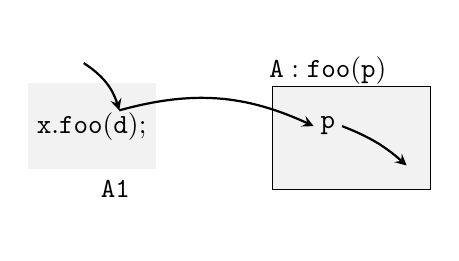
\begin{tikzpicture}
\def\base{1.5}
\def\x{3.0}
\def\xfd{0}
\draw [fill=black!5] (\base + \x + 1.3,0.5) rectangle (\base + \x - 0.7,-.8);
\node[minimum size=11mm] (cs) at (\base + \x, 0.7) {$\mathtt{A:foo(p)}$};
\node[minimum size=11mm, fill=black!5] (cs) at (\base + 0, 0 + \xfd) {$\mathtt{x.foo(d);}$};
\node[minimum size=11mm] (A) at (\base + 0.3, \xfd -.8) {$\mathtt{A1}$};
\node[minimum size=11mm] (p) at (\base + \x, 0) {$\mathtt{p}$};

% edges
\path[-stealth] (\base - 0.1, .8) edge [sloped, thick, bend left=20] (\base + 0.35, 0.2 + \xfd); % ... to d
\path[-stealth] (\base + 0.35, 0.2 + \xfd) edge [sloped, thick, bend left=20] (\base + \x - 0.18, 0.0); % d to p
\path[-stealth] (\base + \x + 0.18, 0.0) edge [sloped, thick, bend left=10] (\base + \x + 1, -
0.5); % p to ...
\end{tikzpicture}
}
        \vspace{-2ex}
        % \caption{Traditional CFL with pre-build call graph}
        \caption{Parameter passing without dispatch}
        \label{fig:approach0}
    \end{subfigure}
        \hspace{-2ex}
    \begin{subfigure}{.32\linewidth}
    \centering
    \resizebox{0.7\width}{0.7\height}{
        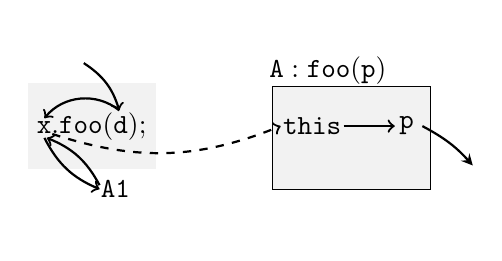
\begin{tikzpicture}
\def\base{1.5}
\def\x{3.0}
\def\xfd{0}
\draw [fill=black!5] (\base + \x + 1.3,.5) rectangle (\base + \x - 0.7,-.8);
\node[minimum size=11mm] (cs) at (\base + \x, .7) {$\mathtt{A:foo(p)}$};
\node[minimum size=11mm, fill=black!5] (cs) at (\base + 0, 0 + \xfd) {$\mathtt{x.foo(d);}$};
\node[minimum size=11mm] (A) at (\base + 0.3, \xfd - .8) {$\mathtt{A1}$};
\node[minimum size=11mm] (this) at (\base + \x - 0.2, 0) {$\mathtt{this}$};
\node[minimum size=11mm] (p) at (\base + \x + 1, 0) {$\mathtt{p}$};

% edges
\path[->] (\base -0.6, -0.15 + \xfd) edge [\colorb, thick, sloped, bend right=20] (\base + 0.1, -.8 + \xfd); % x to A
\path[->] (\base + 0.10, -0.75 + \xfd) edge [\colorc, sloped, thick, bend right=20] (\base -0.57, -0.15 + \xfd); % A to x

%\path[->] (0.1, -2.8) edge [sloped] (3.8, -0.2); % A to p
\path[->] (\base - 0.1, .8) edge [sloped, thick, bend left=20] (\base + 0.35, 0.2 + \xfd); % ... to d
\path[->] (\base + 0.35, 0.2 + \xfd) edge [\colora,sloped, thick, bend right=45] (\base -0.6, 0.1 + \xfd); % d to x 
\path[->] (\base -0.5, -0.1 + \xfd) edge [\colord, dashed, sloped, thick, bend right=20] (\base + \x - 0.6, 0.0); % x to this 
\path[->] (\base + \x + 0.2, 0) edge [sloped, thick] (\base + \x + 0.85, 0.0); % this to p 
\path[-stealth] (\base + \x + 1.2, 0.0) edge [sloped, thick, bend left=10] (\base + \x + 1.84, -
0.5); % p to ...
\end{tikzpicture}
}
        % \caption{New CFL with build-in call graph building}
        \vspace{-2ex}
        \caption{Dispatch at callsite}
        \label{fig:approach1}
    \end{subfigure}
    \hspace{-2ex}
    \begin{subfigure}{.32\linewidth}
    \centering
    \resizebox{0.7\width}{0.7\height}{
        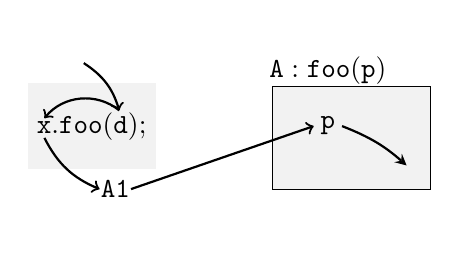
\begin{tikzpicture}
\def\base{1.5}
\def\x{3.0}
\def\xfd{0}
\draw [fill=black!5] (\base + \x + 1.3,.5) rectangle (\base + \x - 0.7,-.8);
\node[minimum size=11mm] (cs) at (\base + \x, .7) {$\mathtt{A:foo(p)}$};
\node[minimum size=11mm, fill=black!5] (cs) at (\base + 0, 0 + \xfd) {$\mathtt{x.foo(d);}$};
\node[minimum size=11mm] (A) at (\base + 0.3, \xfd -.8) {$\mathtt{A1}$};
\node[minimum size=11mm] (p) at (\base + \x, 0) {$\mathtt{p}$};

% edges
\path[->] (\base -0.6, -0.15 + \xfd) edge [\colorb, thick, sloped, bend right=20] (\base + 0.1, -.8 + \xfd); % x to A
\path[->] (\base + 0.5, -.8 + \xfd) edge [\colord, sloped, thick] (\base + \x - 0.18, 0.0); % A to p
\path[-stealth] (\base + \x + 0.18, 0.0) edge [sloped, thick, bend left=10] (\base + \x + 1, -
0.5); % p to ...
\path[->] (\base-0.1, .8) edge [sloped, thick, bend left=20] (\base + 0.35, 0.2 + \xfd); % ... to d
\path[->] (\base + 0.35, 0.2 + \xfd) edge [\colora,sloped, thick, bend right=45] (\base -0.6, 0.1 + \xfd); % d to x 
\end{tikzpicture}
}
        % \caption{CFL with build-in call graph building (dispatch on receiver object)}
        \vspace{-2ex}
        \caption{Dispatch at allocation site}
        \label{fig:approach2}
    \end{subfigure}
%   \vspace{-1.5ex}
    \caption{Three approaches for performing dynamic dispatch at a virtual callsite
    during parameter passing.}
    \label{fig:approach}
 %     \vspace{-2ex}
\end{figure*}

Below we discuss three possible dynamic dispatch approaches, illustrated in \Cref{fig:approach},  for handling parameter passing and explain why \LF is
designed to adopt a callsite-based approach (\Cref{fig:approach1}). 

As discussed in ~\Cref{subsubsec:manuLFC},  \manuLFC~\cite{sridharan2006refinement} solves
\kcs{k} by using a separate algorithm for call graph
construction (\Cref{fig:approach0}) and may thus cause \kcs{k} to lose precision 
(either directly (Sec.~\ref{sec:manuLFC+pre} and Sec.~\ref{sec:LFC+fly}) or  resorting to
a pre-analysis \cite{lu2021selective} (discussed in Sec.~\ref{sec:manuLFC+sep} and evaluated in \Cref{sec:evaluation})).

%The algorithm-assisted dispatching approach \cite{sridharan2005demand, sridharan2006refinement} in such case initiates and on-demand points-to analysis for the receiver variable and once its points-to information is obtained, the dispatching could be proceeded smoothly. 


In  \LF, passing an argument \texttt{d} at \texttt{x.foo(d)}  to a parameter will trigger
immediately a $\iflowsto$ traversal  looking for a
receiver object  of \texttt{x}, as symbolized by a red arrow (\textcolor{\colorb}{$\rightarrow$}) in \Cref{fig:approach1} (for performing dynamic dispatch at this callsite) and \Cref{fig:approach2} (for performing dynamic dispatch at the allocation site of the receiver object). 
\LF adopts the former approach
%(as described in Sec.~\ref{paragraph:chl1} and Sec.~\ref{paragraph:chl2} ) 
since the latter is infeasible.

Let us explain why the allocation-site-based dispatch (\Cref{fig:approach2}) is infeasible.
To handle parameter passing only (without considering method returns here), we need to extend \manuLF to become:
\begin{equation} 
% \footnotesize
\label{eqn:newFlows}
\begin{tabular}{rcl} 
$\flows$ & $\longrightarrow$ & $\cdots \mid \store[\texttt{m:i}]\ \iflowsto\ \load[\texttt{m:i}]$\\
$\iflows$ & $\longrightarrow$ &  $\cdots \mid  \iloadfield{\texttt{m:i}} \ \iflowsto \ \istorefield{\texttt{m:i}}$
\end{tabular}
\end{equation}
where  $\store[\texttt{m:i}]$ ($\load[\texttt{m:i}]$) is used to replace
 $\store[\texttt{i}]$ ($\load[\texttt{i}]$) in \Cref{fig:newcflpag}  in order
 to encode also the  signature of a method invoked at 
 $\mathtt{r}.\mathtt{m}(a_1, \dots, a_n)$. Thus, the \manuLFC-path in \Cref{eq:LFCPathCGPreciseI}
becomes:
%{
% \addtolength\abovedisplayskip{-.5ex}
% \addtolength\belowdisplayskip{-1.5ex}
\begin{equation} 
\footnotesize
  \centering
\label{eq:alterLFPath}
\begin{tabular}{l} 
\commentfont{O1}$\xrightarrow{\new}
\texttt{o1}\xrightarrow[\hat{\mathtt{c1}}]{\assign}
\texttt{o} \xrightarrow{\store[\texttt{f}]} \texttt{d}
\xrightarrow{\inew}$ 
\commentfont{D1} 
$ \xrightarrow{\new} \texttt{d}$ $\xrightarrow{\store[\texttt{foo:1}]}\texttt{x}\xrightarrow[\check{\mathtt{c1}}]{\iassign}\texttt{a}
\xrightarrow{\inew}$\commentfont{A1}$\xrightarrow{\load[\texttt{foo:1}]}\texttt{p}
    \xrightarrow{\load[\texttt{f}]} \texttt{v}
$
% \\[3ex]
% \begin{tikzpicture}[-, remember picture,overlay]
% \def\lx{6.2}\def\ly{.99}
% \def\dy{.54}\def\ny{.07}
% \draw(\lx, \ly) -- (\lx+.1, \ly) -- (\lx+.1, \dy);
% \draw[dashed] (\lx+.1, \dy) -- (-.12,\dy);
% \draw(-.12,\dy) -- (-.12, \ny);
% \draw[->] (-.12, \ny) -- (0.06, \ny);
% \end{tikzpicture}
% \footnotesize
\end{tabular}
\end{equation}
%}
where we have
$\texttt{d}\xrightarrow{\store[\texttt{foo:1}]}\texttt{x}$
(\textcolor{\colora}{$\rightarrow$}), 
$\texttt{x} \xrightarrow[\check{\mathtt{c1}}]{\iassign}\texttt{a} \xrightarrow{\inew}$\commentfont{A1}
(\textcolor{\colorb}{$\rightarrow$}), and
\commentfont{A1}$\xrightarrow{\load[\texttt{foo:1}]}\texttt{p}$
(\textcolor{\colord}{$\rightarrow$}). However, 
 \commentfont{O1} flows to \texttt{v} under \emptyctx incorrectly (with
$\hat{\texttt{c1}}$ and $\check{\texttt{c1}}$ being matched). \hl{Due to the
nature of object-sensitivity (where receiver objects are used as context elements)},
 the CFL-reachability formulation for object-sensitive pointer analysis \cite{lu2019precision, lu2021eagle} (as reviewed briefly in \Cref{sec:relatedwork:cfl}) works well with the allocation-site-based dispatch approach.



% There seems to be another choice here. 
% In the above process, when we find the receiver object, we have gathered all the information needed for dispatching. One would ask why we must go back to the callsite. It is true if only context-insensitive analysis is considered. For example, we can use \argrec to mark the beginning of searching for a receiver object. After we find the specific object, we need to know which callsite (to be precise, its method signature) is being processed to dispatch correct method according to the type and method signature. We also need to know which parameter is being passed in order to pass the correct parameter after dispatch. This can be solved by adding a set of balanced parentheses with method signature and parameter: When we start looking for receiver object at \argrec, we introduce the method signature of the callsite and the target parameter on the stack. That is, \argrec[m:i]. After finding the specific object, we can match it with, say, \recparm[m:i] to pass the argument to the correct formal parameter, which can be established statically. That is, the previous "entry" edge in \rulename{P-Call} is parsed with \argrec[m:i] \iflowsto \recparm[m:i] rather than a simple \assign edge as before. And the non-terminal \flows in \cref{eqn:callsiteLF} is changed to:

% "exit" edge in \rulename{P-Call} and \iflows in \cref{eqn:callsiteLF} should be changed accordingly but omitted here. The process of this kind of way of handling of parameter passing is illustrated in \cref{fig:approach1}.


%However, the context after the parameter passing is different from the traditional formulation \cite{sridharan2005demand, sridharan2006refinement}. Consider the following flow path from 
%\commentfont{O1} to \texttt{v} in \Cref{fig:motivatingExample} (again but this time expressed by $\mathcal{L}_{F'C}$ as \Cref{eq:alterLFPath}):

% For example, if we simply apply \cref{eqn:newFlows}, we will find that although we can find the correct formal parameter for this single parameter passing, the context for \texttt{p} or \texttt{v} after the parameter passing is not as expected. We note the language $L_F$ modified with \cref{sec:newFlows} as $L_{F'}$. The path from \commentfont{O1} to 
% \texttt{v} is expressed by $L_{FC}$ as \cref{eq:LFCPathCGPreciseI} but is expressed by $L_{F'C}$ as \cref{eq:alterLFPath}:
\begin{comment}
The $L_C(p_{\color{purple}{\mathtt{O1}},\texttt{v}})=\hat{\mathtt{c1}}\hat{\mathtt{c3}}$ in \Cref{eq:LFCPathCGPreciseI} but \LC$(p_{\color{purple}{\mathtt{O1}},\texttt{v}})=\hat{\mathtt{c1}}\check{\mathtt{c1}}$ in \Cref{eq:alterLFPath}, resulting in 
inconsistent calling contexts for \texttt{v} (i.e., $[\mathtt{c3}, \mathtt{c1}]$ and \emptyctx ~ respectively) when the parameter passing is completed.
\end{comment}
%We know that the callsite-sensitivity is modeling call stacks, so $\mathcal{L}_{F'C}$ is incorrect
%for a callsite-sensitive analysis. 
%Note that attempting to encode context information into below-edges in \pag (e.g., replacing $\xrightarrow{\load[\texttt{foo:1}]}$ in \Cref{eq:alterLFPath} with $\xrightarrow[\hat{\texttt{c1}};\hat{\texttt{c3}}]{\load[\texttt{foo:1}]}$) is also infeasible as one method may be invoked under different calling contexts with a same receiver object and statically establishes \LC strings from receiver variables to receiver objects would be another challenge. 

%By returning to the callsite after finding the receiver object, changing the dispatching location to callsite, and together with the following \LR, \challenge{3} can be addressed.


\subsubsection{The $L_R$ Language}
\label{subsubsec:newLR}

%Given \LF (defined in \Cref{eqn:finalNewLF}) and $\LC=\manuLC$ (defined in \Cref{eqn:callsiteLC}), we have obtained a new language: \capLFC. However,
%\LFC solves \kcs{k} soundly but less precisely than \manuLFCDD (Lemma~\ref{thm:lfc-imprecise}).

\LFC is sound but imprecise. We  use two examples given in
\Cref{fig:LFC-imprecision-callsite} and \Cref{fig:LFC-imprecision-context} to illustrate the imprecision of \LFC and highlight the two roles that \LR plays
in \LFCR. 

\LFC can lose precision caused by an incorrect  dispatch callsite. Consider the following two \LFC-paths in the PAG of \Cref{fig:LFC-imprecision-callsite} (by ignoring  the boxed labels $\hat{\boxed{\texttt{c1}}}$, $\check{\boxed{\texttt{c1}}}$ and $\check{\boxed{\texttt{c2}}}$ for now):
\begin{equation} 
\label{eq:ex2-inv-c1-site}
  \centering
\begin{tabular}{l} 
\commentfont{O1}$\xrightarrow{\new[\texttt{O}]} \texttt{o1} 
\xrightarrow[\hat{\boxed{\texttt{c1}}}]{\store[1]} \texttt{a} 
\xrightarrow{\inewfield{\texttt{A}}}
$
\commentfont{A1}
$ \xrightarrow{\new[\texttt{A}]} \texttt{a}$
$\xrightarrow[\check{\boxed{\texttt{c1}}}]{\assign} \texttt{a\#c1}
\xrightarrow[\hat{\texttt{c1}}]{\indispatch[\texttt{A}]} \texttt{this}^{\texttt{m}} 
\xrightarrow{\load[1]} \texttt{p}
$
\end{tabular}
\end{equation}

%\bigskip
\vspace*{-1ex}

\begin{equation} 
\label{eq:ex2-inv-c2-site}
  \centering
\begin{tabular}{l} 
\commentfont{O1}$\xrightarrow{\new[\texttt{O}]} \texttt{o1} 
\xrightarrow[\hat{\boxed{\texttt{c1}}}]{\store[1]} \texttt{a} 
\xrightarrow{\inewfield{\texttt{A}}}
$
\commentfont{A1}
$ \xrightarrow{\new[\texttt{A}]} \texttt{a}$
$\xrightarrow[\check{\boxed{\texttt{c2}}}]{\assign} \texttt{a\#c2}
\xrightarrow[\hat{\texttt{c2}}]{\indispatch[\texttt{A}]} \texttt{this}^{\texttt{n}} 
\xrightarrow{\load[1]} \texttt{q}
$
\end{tabular}
\end{equation}

These two \LFC-paths both keep track of where \commentfont{O1}  flows to in the
\pag of this program.
According to the first \LFC-path, \commentfont{O1} flows to \texttt{p} as 
expected. However, due to the existence of the second \LFC-path, 
\commentfont{O1} can also flow to \texttt{q} spuriously as the $\iflowsto$ traversal for finding the receiver object of \texttt{a} is triggered at callsite \texttt{c1} but the dispatch ends up happening at  callsite \texttt{c2}. To eliminate such precision loss, \LR requires  boxed edge labels to be matched as balanced parentheses. As a result,  the first \LFC-path in \Cref{eq:ex2-inv-c1-site} will be considered
as a valid \LFCR-path (since $\hat{\boxed{c1}}$ is matched by $\check{\boxed{c1}}$) but  the second \LFC-path in \Cref{eq:ex2-inv-c2-site} will be ruled out (since $\hat{\boxed{c1}}$ is not matched by $\check{\boxed{c2}}$). 

\LFC can also lose precision caused by an incorrect dispatch context.  
Consider the following two \LFC-paths in the PAG of \Cref{fig:LFC-imprecision-context}
(by ignoring  the boxed labels $\hat{\boxed{\texttt{c3}}}$ and $\check{\boxed{\texttt{c3}}}$ 
for now):


\begin{figure}
\begin{mdframed}[
align=center,
usetwoside=false,
 rightmargin=3cm,
innerleftmargin=1.0ex,
innerrightmargin=-20.0ex
innertopmargin=0.2ex,
innerbottommargin=0.2ex
]

\begin{minipage}{0.4\linewidth}
\begin{lstlisting}[language=java, basicstyle=\linespread{0.8}]
static void main() {
  A a = new A(); // A1
  O o1 = new O(); // O1
  O o2 = new O(); // O2
  a.m(o1); // c1
\end{lstlisting}
\end{minipage}
\hspace{-2ex}
\begin{minipage}{0.4\linewidth}
\begin{lstlisting}[language=java, firstnumber=6, basicstyle=\linespread{0.8}]
  a.n(o2); } // c2
class O { }
class A {
  void m(Object p) { ... }
  void n(Object q) { ... } }
\end{lstlisting}
\end{minipage}

\end{mdframed}
\caption{An example for illustrating the imprecision of \LFC caused by an
incorrect dispatch site.
    \label{fig:LFC-imprecision-callsite}}
\end{figure}



\begin{figure}
\begin{mdframed}[
align=center,
usetwoside=false,
rightmargin=3cm,
innerleftmargin=1.0ex,
innerrightmargin=-20.0ex
innertopmargin=0.2ex,
innerbottommargin=0.2ex
]

\begin{minipage}{0.4\linewidth}
\begin{lstlisting}[language=java, basicstyle=\linespread{0.8}]
class A {
  O id(O p) { return p; } }
class O { }
static O wid(A a, O o) {
  O v = a.id(o); // c3
  return v;
}
\end{lstlisting}
\end{minipage}
\hspace{-2ex}
\begin{minipage}{0.4\linewidth}
\begin{lstlisting}[language=java, firstnumber=8, basicstyle=\linespread{0.8}]
static void main() {
  A a1 = new A(); // A1
  O o1 = new O(); // O1
  O o2 = new O(); // O2
  O v1 = wid(a1, o1); // c1
  O v2 = wid(a1, o2); // c2
}
\end{lstlisting}
\end{minipage}
\end{mdframed}
\caption{An example for illustrating the imprecision of \LFC caused by an
incorrect dispatch context.
    \label{fig:LFC-imprecision-context}}
\end{figure}

\begin{equation} 
% \scriptsize
\label{eq:ex2-inv-c1}
  \centering
\begin{tabular}{l} 
\commentfont{O1}$\xrightarrow{\new[\texttt{O}]} \texttt{o1}
\xrightarrow[\hat{\texttt{c1}}]{\assign} \texttt{o} 
\xrightarrow[\hat{\boxed{\texttt{c3}}}]{\store[1]} \texttt{a} 
\xrightarrow[\check{\texttt{c1}}]{\iassign} \texttt{a1}
\xrightarrow{\inewfield{\texttt{A}}}
$
\commentfont{A1}
$ \xrightarrow{\new[\texttt{A}]} \texttt{a1} 
\xrightarrow[\hat{\texttt{c1}}]{\assign} \texttt{a}$ \\[5ex]
\begin{tikzpicture}[-, remember picture,overlay]
\def\lx{10.4}\def\ly{1.4}
\def\dy{.76}\def\ny{.065}
\draw(\lx, \ly) -- (\lx+.1, \ly) -- (\lx+.1, \dy);
\draw[dashed] (\lx+.1, \dy) -- (-.12,\dy);
\draw(-.12,\dy) -- (-.12, \ny);
\draw[->] (-.12, \ny) -- (0.06, \ny);
\end{tikzpicture}
$\xrightarrow[\check{\boxed{\texttt{c3}}}]{\assign} \texttt{a\#c3}
\xrightarrow[\hat{\texttt{c3}}]{\indispatch[\texttt{A}]} \texttt{this}^{\texttt{id}} 
\xrightarrow{\load[1]} \texttt{p} \xrightarrow{\store[\ret]} \texttt{this}^{\texttt{id}} 
\xrightarrow[\check{\texttt{c3}}]{\iindispatchfield{\texttt{A}}} \texttt{a\#c3}
$ \\[5ex]
\begin{tikzpicture}[-, remember picture,overlay]
\def\lx{10.4}\def\ly{1.4}
\def\dy{.76}\def\ny{.065}
\draw(\lx, \ly) -- (\lx+.1, \ly) -- (\lx+.1, \dy);
\draw[dashed] (\lx+.1, \dy) -- (-.1,\dy);
\draw(-.12,\dy) -- (-.12, \ny);
\draw[->] (-.12, \ny) -- (0.06, \ny);
\end{tikzpicture}
$\xrightarrow[\hat{\boxed{\texttt{c3}}}]{\iassign} \texttt{a}
\xrightarrow[\check{\texttt{c1}}]{\iassign} \texttt{a1} 
\xrightarrow{\inewfield{\texttt{A}}}$
\commentfont{A1}$\xrightarrow{\new[\texttt{A}]} \texttt{a1}
\xrightarrow[\hat{\texttt{c1}}]{\assign} \texttt{a}
\xrightarrow[\check{\boxed{\texttt{c3}}}]{\load[\ret]}
\texttt{v} \xrightarrow[\check{\texttt{c1}}]{\assign} 
\texttt{v1}
$
\end{tabular}
\end{equation}

\bigskip

\begin{equation} 
% \scriptsize
\label{eq:ex2-inv-c2}
  \centering
\begin{tabular}{l} 
\commentfont{O1}$\xrightarrow{\new[\texttt{O}]} \texttt{o1}
\xrightarrow[\hat{\texttt{c1}}]{\assign} \texttt{o} 
\xrightarrow[\hat{\boxed{\texttt{c3}}}]{\store[1]} \texttt{a} 
\xrightarrow[\check{\texttt{c1}}]{\iassign} \texttt{a1}
\xrightarrow{\inewfield{\texttt{A}}}
$
\commentfont{A1}
$ \xrightarrow{\new[\texttt{A}]} \texttt{a1} 
\xrightarrow[\hat{\texttt{c2}}]{\assign} \texttt{a}$ \\[5ex]
\begin{tikzpicture}[-, remember picture,overlay]
\def\lx{10.4}\def\ly{1.4}
\def\dy{.76}\def\ny{.065}
\draw(\lx, \ly) -- (\lx+.1, \ly) -- (\lx+.1, \dy);
\draw[dashed] (\lx+.1, \dy) -- (-.12,\dy);
\draw(-.12,\dy) -- (-.12, \ny);
\draw[->] (-.12, \ny) -- (0.06, \ny);
\end{tikzpicture}
$\xrightarrow[\check{\boxed{\texttt{c3}}}]{\assign} \texttt{a\#c3}
\xrightarrow[\hat{\texttt{c3}}]{\indispatch[\texttt{A}]} \texttt{this}^{\texttt{id}} 
\xrightarrow{\load[1]} \texttt{p} \xrightarrow{\store[\ret]} \texttt{this}^{\texttt{id}} 
\xrightarrow[\check{\texttt{c3}}]{\iindispatchfield{\texttt{A}}} \texttt{a\#c3}
$ \\[5ex]
\begin{tikzpicture}[-, remember picture,overlay]
\def\lx{10.4}\def\ly{1.4}
\def\dy{.76}\def\ny{.065}
\draw(\lx, \ly) -- (\lx+.1, \ly) -- (\lx+.1, \dy);
\draw[dashed] (\lx+.1, \dy) -- (-.1,\dy);
\draw(-.12,\dy) -- (-.12, \ny);
\draw[->] (-.12, \ny) -- (0.06, \ny);
\end{tikzpicture}
$\xrightarrow[\hat{\boxed{\texttt{c3}}}]{\iassign} \texttt{a}
\xrightarrow[\check{\texttt{c2}}]{\iassign} \texttt{a1} 
\xrightarrow{\inewfield{\texttt{A}}}$
\commentfont{A1}$\xrightarrow{\new[\texttt{A}]} \texttt{a1}
\xrightarrow[\hat{\texttt{c2}}]{\assign} \texttt{a}
\xrightarrow[\check{\boxed{\texttt{c3}}}]{\load[\ret]}
\texttt{v} \xrightarrow[\check{\texttt{c2}}]{\assign} 
\texttt{v2}
$
\end{tabular}
\end{equation}

These two \LFC-paths differ only in their underlying contexts  and  target variables used:
the second  can be obtained from the first by
replacing each occurrence of \texttt{c1} with \texttt{c2} and \texttt{v1} with \texttt{v2}.
Both \LFC-paths  keep track of where \commentfont{O1} will flow to,
starting from the call ``\inline{wid(a1,o1); // c1}''. According to the first
\LFC-path,  \texttt{v1} points to \commentfont{O1} as
expected. However, due to the existence of the second \LFC-path, 
\commentfont{O1}, which comes from callsite \texttt{c1}, will flow into \texttt{v2} at callsite \texttt{c2} spuriously.
Consider the dynamic dispatch that happens at ``\inline{a.id(o); // c3}''
due to the call\linebreak  ``\inline{wid(a1,o1); // c1}''. 
In the first \LDC-path,
\texttt{a} starts with pointing to \commentfont{A1} under
 [\texttt{c1}]
 during its $\iflowsto$  traversal (to find what \texttt{a} points to)
 and ends up with pointing  to \commentfont{A1} under  
  [\texttt{c1}] during
 the ensuing
 $\flowsto$ traversal.
 This $\flowsto$ traversal can
 happen from the call  ``\inline{wid(a1,o1); // c1}''. However, in the second \LDC-path,
\texttt{a} starts also with pointing to \commentfont{A1} under
 [\texttt{c1}]
 during its $\iflowsto$  traversal but ends up with pointing  to \commentfont{A1} under  
  [\texttt{c2}] during
 the ensuing
 $\flowsto$ traversal. This  $\flowsto$ traversal cannot
 happen from the call  ``\inline{wid(a1,o1); // c1}''.

\begin{comment}
In both \LFC-paths,  the same $\iflowsto$  traversal is performed to find that
\texttt{a}  points to \commentfont{A1} under $\CC=[\texttt{c1}]$. However,
when returning to \texttt{a} during the following
 $\flowsto$ traversal, we traverse the same $\iflowsto$-path backwards
 under also $[\texttt{c1}$] (which can happen under under $\CC=[\texttt{c1}$]
 in the first \LFC-path but 
 and
 ends up with pointing  to \commentfont{A1} under also 
  [\texttt{c1}] during
  (which is possible under $\CC=[\texttt{c1}$]. 
 


This path contains two dispatch paths for ``\inline{a.id(o) // c3}'', 
one for  passing \texttt{o} to \texttt{p} and one for returning 
 \texttt{p} back to the same callsite. 
The first one is invalid, since \texttt{a} starts with pointing to \commentfont{A1} under
 [\texttt{c1}]
 during its $\iflowsto$  traversal but ends up with pointing  to \commentfont{A1} under  
  [\texttt{c2}] during
 the ensuing
 $\flowsto$ traversal, violating \dispatchconTwo. Thus, \LFC enables
 \commentfont{O1} passed at callsite \texttt{c1} to flow into \texttt{v2}
 at callsite \texttt{c2}  spuriously.
\end{comment}

Consider a virtual callsite 
``$\mathtt{r}.\mathtt{m}(a_1, \dots, a_n); ~ // \mathtt{c}$'' with a reference to
\Cref{eq:proof-valid-DP}.
In general, when performing a $\iflowsto$ traversal to find that 
$\mathtt{r}$ points to a receiver object $O$ under $[\check{c_1},...,\check{c_k}]$,
\LR must be designed to ensure that we can return from $O$ to $\mathtt{r}$  by performing a $\flowsto$ traversal
under exactly $[\hat{c_k},...,\hat{c_1}]$ in order to avoid passing arguments spuriously.

To address \challenge{3} (i.e., the two sources of imprecision above), we  introduce  a third CFL \LR: 
\begin{equation}
\footnotesize
    \label{eqn:callsiteLR}
    \begin{tabular}{rcl}
$\recoveredctx$ & $\longrightarrow$ & $\recoveredctx~\hat{c} \mid \recoveredctx~\check{c} \mid \recoveredctx~ \siterecovered \mid \epsilon$\\[1ex]
$\siterecovered$ & $\longrightarrow$ & $\hat{\boxed{c}} ~ \ctxrecovered ~ \check{\boxed{c}}$\\[1ex]
$\ctxrecovered$ & $\longrightarrow$ & $\matched ~ \ctxrecovered \mid \ctxrecovered ~ \matched \mid\check{c} ~ \ctxrecovered ~ \hat{c} \mid \epsilon$\\[1ex]
$\matched$ & $\longrightarrow$ & $\matched ~ \matched \mid \hat{c} ~ \matched ~ \check{c} \mid \siterecovered\mid\epsilon$ \\[1ex]
    \end{tabular}
\end{equation}
%where its terminals are the below-edge labels, $\hat{c}$ and$\check{c}$, $\hat{\boxed{c}}$, and $\check{\boxed{c}}$, in the \pag. 

All the above-edge labels are handled similarly as in the case of \manuLC. By
decomposing each double-label edge into a sequence of
two single-label edges as described in
\Cref{subsubsec:CFLReachability}, $\matched$ is extended by adding
a new production 
$\matched \longrightarrow  \reg{above-edge-label}$, where
 the new non-terminal
\reg{above-edge-label}  is defined in terms of all the original above-edge
labels  in a given \pag.


With \LR being incorporated into
\LFC, the resulting language \capLFCR will be precise in handing parameter passing for virtual callsites. Let us return  to  the two paths given in \Cref{eq:ex2-inv-c1} and
\Cref{eq:ex2-inv-c2} with  $\hat{\boxed{\texttt{c3}}}$
and $\check{\boxed{\texttt{c3}}}$) being considered.
The first one is an \LFCR-path but the second is not. 
The first one is an  \LFCR-path, since we start the dynamic dispatch process
at callsite \texttt{c3} (marked by the first 
  $\hat{\boxed{\texttt{c3}}}$)
under context $[\texttt{c1}]$ and return to the same callsite under
the same context at the end of this dynamic dispatch process (marked by the first
  $\check{\boxed{\texttt{c3}}}$) even though \texttt{c1} is lost, i.e.,
  balanced out due to 
  $\hat{{\texttt{c1}}}\check{{\texttt{c1}}}$ just after the first
  $\mathtt{a}\xrightarrow[\check{{\mathtt{c1}}}]{\iassign} \mathtt{a1}$ edge is
  traversed.
  The second one is \emph{not} an  \LFCR-path, since even though we also start the dynamic dispatch process
at callsite \texttt{c3} (marked by the first 
  $\hat{\boxed{\texttt{c3}}}$)
under context $[\texttt{c1}]$, we end up returning to the same callsite under
a different and thus incorrect context, $[ \texttt{c2}]$, at the end of this dynamic dispatch process (marked by the first
  $\check{\boxed{\texttt{c3}}}$).
  %once \texttt{c1} is    balanced out due to   $\hat{{\texttt{c1}}}\check{{\texttt{c1}}}$ just after the first  $\mathtt{a}\xrightarrow[\check{{\mathtt{c1}}}]{\iassign} \mathtt{a1}$ edge is  traversed.
As a result, \LFCR will conclude that
\commentfont{O1} is pointed to by \texttt{v1} but not by \texttt{v2} as desired.

Below, we give a formal development of \LR  and then
prove the precision of \LFCR.

We can obtain the points-to set of a variable $v$,  $\pointsto(v, c_v)$,
from \LFC as follows. 
Given an \LC-path $p$ with its label being
$\LC(p)=\ell_1,\dots,\ell_n$, where each $\ell_i$ is an entry or exit
context label in an inter-procedural \assign edge,
%(implying that  $\LC(p)\in\LC$),  
 the inverse of $p$, i.e.,
$\overline{p}$ has the label
$\LC(\overline{p})=\overline{\ell_n},\dots,
\overline{\ell_1}$.
% (implying that  $\LC(\overline{p})\in\LC$). 
By splitting $p$ into a sub-path $p^\exit$ followed
by a sub-path $p^\entry$, we can define $\LC^\exit(p)=\LC(p^\exit)$ 
and $\LC^\entry(p)=\LC(p^\entry)$, where
$\LC(p) = \LC^\exit(p)\LC^\entry(p)$, such that  $\LC^\exit(p)$ ($\LC^\entry(p)$) is
derived from 
\gramexit (\gramentry) in \LC's grammar (\Cref{eqn:callsiteLC}).
Let $s\in \LC$.
Let $\BalParen{s}$ return the canonical form of $s$ with
all its balanced contexts (i.e., parentheses) removed.
If $c$ is a string of exit contexts  of the form
$\check{c_1}
\dots\check{c_n}$, we write 
$\RawCtxCheck{c} = [c_1,\dots,c_n]$ to turn it into a context representation
(by noting that $\RawCtxCheck{\epsilon}=\emptyctx$).



\begin{comment}
Our CFL-reachability formulation
of \kcs{k}, defined by 
\capLFCR, discovers the points-to information in \pag as follows.
A path $p$ from $O$ to $v$ in \pag can be identified as a context-sensitive \flowsto relation iff $p$ is both (1) a $\flowsto$ path in \LF, where  $O\;\flowsto\; v$, (2) a realizable path in \LC, where 
$\realizable \Longrightarrow^* \mathcal{L}_C(p)$, and (3) a $W$ path in \LR, where $W \Longrightarrow^* \mathcal{L}_R(p)$, yielding the following
context-sensitive points-to relation:
\end{comment}

Given an \LFC-path  $p$ starting from an object $O$ to a variable $v$, we can deduce the following points-to relation with the contexts of $O$ and $v$ being spelt out clearly:
%{
%\addtolength\abovedisplayskip{-.3ex}
%\addtolength\belowdisplayskip{-.3ex}
\begin{equation}
\label{eq:pt-ctx}
%\hspace*{-1ex}
\begin{tabular}{@{}r@{\ }c@{\ }l@{}}
$\langle O,\RawCtxCheck{\BalParen{\LC^\exit(p)}}\rangle$ & $\quad\in \quad$  &
$\pointsto(v, \RawCtxHat{\overline{\BalParen{\LC^\entry(p)}}}
)$\\
\end{tabular}
\end{equation}

\begin{comment}
where
\begin{eqnarray}
\label{eq:pt-ctx}
\begin{tabular}{@{}r@{\ }c@{\ }l@{}}
$ctx(\mathcal{L}_C^\entry(p))$ & $\eqdef$ & sequence of unbalanced  $\check{c}$\,'s in\\&& $\overline{\mathcal{L}_C^\entry(p)}$ with their hats elided;\\
$ctx(\mathcal{L}_C^\exit(p))$ & $\eqdef$ & sequence of  unbalanced  $\check{c}$\,'s in\\&&  
$\mathcal{L}_C^\exit(p)$ with their checks elided.
\end{tabular}
%\hspace*{-3ex}
\end{eqnarray}
\end{comment}
Let us consider an example.
Let $p_{{\color{purple}\texttt{O1}},\texttt{v}}$ be the \LFC-path in \Cref{eq:ex-patho1-to-v} (by 
ignoring
  $\hat{\boxed{\texttt{c3}}}$
and $\check{\boxed{\texttt{c3}}}$). By definition, 
$\LC(p_{{\color{purple} \texttt{O1}},\texttt{v}})=\hat{\texttt{c1}}\check{\texttt{c1}}\hat{\texttt{c1}}
\hat{\texttt{c3}}$, where
$p_{{\color{purple}\texttt{O1}},\texttt{v}}^\exit$ can be interpreted
as the sub-path from \commentfont{O1} to \commentfont{A1} and $p_{{\color{purple} \texttt{O1}},\texttt{v}}^\entry$
as the sub-path from \commentfont{A1} to \texttt{v}. Thus,
$\LC^\exit(p_{{\color{purple}\texttt{O1}},\texttt{v}})  =\hat{\texttt{c1}}\check{\texttt{c1}}$ and $\LC^\entry(p_{{\color{purple}\texttt{O1}},\texttt{v}})=\hat{\texttt{c1}}
\hat{\texttt{c3}}$. Since
$\RawCtxCheck{\BalParen{\hat{\texttt{c1}}\check{\texttt{c1}}}}
=\RawCtxCheck{\epsilon}=\emptyctx$ and
$\RawCtxHat{\overline{\BalParen{\hat{\texttt{c1}}\hat{\texttt{c3}}}}}
=
\RawCtxHat{\overline{{\hat{\texttt{c1}}\hat{\texttt{c3}}}}}
=
\RawCtxHat{{{\check{\texttt{c3}}\check{\texttt{c1}}}}}
=
[{{{{\texttt{c3}},{\texttt{c1}}}}}]
$, we have:
\begin{equation*}
 \langle {\color{purple}\texttt{O1}},\emptyctx \rangle\quad \in\quad
\pointsto(\texttt{v}, [\texttt{c3},\texttt{c1}])
\end{equation*}



\LFC can lose precision  since, for some \LFC-paths, its sub-paths responsible for
performing dynamic dispatch can be spurious. Consider a virtual callsite $ \texttt{r}.\mathtt{m}(a_1, \dots, a_n) ~ //~ c$.  
Before passing an argument $a_i$ into (or receiving a return value from) a
method invoked, \LFC performs dynamic dispatch  
by carrying out
the following alias-related traversal on its receiver variable $\mathtt{r}$:
\begin{equation}
% \footnotesize
\label{eq:dispatchpath}
\cdots \xrightarrow[\hat{\boxed{c}}]{\ell} \mathtt{r} ~
\iflowsto ~ O ~ \flowsto ~\mathtt{r}'
% ~ \alias\quad~ r'
 \xrightarrow[\check{\boxed{c'}}]{\assign} \mathtt{r}'\#c'
 \xrightarrow[\hat{c'}]{\indispatch[\texttt{\_}]}\cdots
 %\texttt{this}^\texttt{T:foo()}
 \end{equation}
 where $\ell$ is $\storefield{i}$ (in passing $a_i$) or $\iloadfield{0}$ (in
 retrieving a return value). Such a path, which starts from 
 $\hat{\boxed{c}}$ and ends at $\check{\boxed{c'}}$, is called 
 a \textit{dispatch path}, which
is \emph{valid} if  two conditions are met:
\begin{itemize}
    \item \dispatchconOne: $c=c'$ (implying that $\mathtt{r}=\mathtt{r}'$), and
%    \item \dispatchconTwo:  $\mathtt{r}$ and $\mathtt{r}'$ are aliased  under   the same context.
    \item \dispatchconTwo: $O$ is pointed by both $\mathtt{r}$ and $\mathtt{r}'$ (which
    are thus aliases) under   exactly the same context.
\end{itemize} 

 However, \LFC can only ensure that $\mathtt{r}$ and $\mathtt{r}'$ are aliases but with no guarantee for the validity of
 this dispatch path.
To filter out all  \LFC-paths containing invalid dispatch paths, we use  \LR 
given earlier
to enforce
\dispatchconOne and \dispatchconTwo, thereby addressing 
\challenge{3} by
restoring  the callsite and context of $\mathtt{r}$. In particular,
 the $\siterecovered$-production  enforces
\dispatchconOne, and the set of $\ctxrecovered$-productions, together with the set of $\matched$-productions, enforce \dispatchconTwo.
% by not only matching method calls and returns as a balanced-parentheses problem but also ensuring contexts to be restored when dispatching:
%\input{languageC.tex}
%{
%\addtolength\abovedisplayskip{-.5ex}
%\addtolength\belowdisplayskip{-.5ex}
% \begin{equation}
% \label{eqn:callsiteLC}
% \footnotesize
%     \begin{split}
% \textsf{realisable} \longrightarrow \textsf{exit} ~ \textsf{entry} \\
% \textsf{exit} \longrightarrow \textsf{exit} ~ \textsf{B} \mid \textsf{exit} \ \check{c} \mid \epsilon \\ 
% \textsf{entry} \longrightarrow \textsf{entry} ~ \textsf{B} \mid \textsf{entry} \ \hat{c} \mid \epsilon \\
% \textsf{B} \longrightarrow \textsf{B} ~ \textsf{B} \mid \hat{c} ~ \textsf{B} ~ \check{c} \mid \hat{\boxed{c}} ~ R ~ \check{\boxed{c}} \mid \epsilon \\
% R \longrightarrow B ~ R \mid R ~ B \mid \check{c} ~ R ~ \hat{c} \mid H\\
% H \longrightarrow B ~ H \mid H ~ B \mid \hat{c} ~ H ~ \check{c} \mid \epsilon\\
%     \end{split}
% \end{equation}

%, with both being mutually recursive due to the recursive nature of \kcs{k}.

%\LR is an supplementary language of \LC for supporting dynamic dispatching. 
%Below, we highlight that how we address \challenge{3} in \LR. 


%\Cref{thm:lfc-imprecise} has shown that \LFC is a superset of \manuLFC, we must show how the extra words are correctly filtered out by \LR.
%happens under  the same context as in the
%\manuLFC-based formulation (with dynamic dispatch done separately), by exploiting the balanced matching property of virtual call dispatching.
\begin{comment}
By construction, \LFC enforces that we find receiver object from the receiver variable of a callsite (say, $x$ on $c$) and return to the receiver variable of a callsite (say, $x'$ on $c'$). But it only ensures $x$ and $x'$ are alias. It guarantees neither $c$ and $c'$ are same nor $x$ and $x'$ are context-sensitively the same variable (under the same context). This can be respectively addressed in two cases: {\bf case 1.} By using a balanced parentheses matching of $\hat{\boxed{c}}$ and $\check{\boxed{c}}$, we guarantee $c$ and $c'$ are same. {\bf case 2.} The production rule for non-terminal $Y$ between $\hat{\boxed{c}}$ and $\check{\boxed{c}}$ enforces we start and end at the same receiver variable. Below, we discuss it in details.
\end{comment}
%As stated earlier in \LF, we require that $\store[\texttt{i}]$ matched by $\load[\texttt{i}]$ and type $\texttt{t}$ in $\indispatch[\texttt{t}]$
%must be consistent with the one in $\new[\texttt{t}]$ of current $\flowsto$ value flow. However, these could not guarantee that dispatching is correct as we have chosen to perform dispatching at callsites (\Cref{fig:approach2}).

\begin{comment}


\paragraph{Imprecision of \LFC}
\label{sec:LFC-impre}

We look at two  examples  to understand why \LFC fails to enforce
\dispatchconOne and \dispatchconTwo. 

Consider the following simple code snippet:
%where \texttt{A} is modified by adding a new method definition ``\lstinline[language=java]!void goo(D s){}!''):
\vspace{.5ex}
\begin{mdframed}[
%innermargin =-2ex,
%  rightmargin=-1cm,
innerleftmargin=-0.3ex,
innerrightmargin=-1.0ex,
innertopmargin=0.0ex,
innerbottommargin=0.2ex
]
\begin{lrbox}{\mybox}
\begin{lstlisting}[language=java, basicstyle=\linespread{0.8}\small, numbers=none]
D d1 = new D(); // D1
D d2 = new D(); // D2
A a = new A(); // A1
a.foo(d1); // c1
a.foo(d2); // c2
\end{lstlisting}
\end{lrbox}
\scalebox{0.9}{\usebox{\mybox}}
\end{mdframed}
where classes \texttt{A} and \texttt{D} are from \Cref{fig:motivatingExample}.
The following path is accepted by \LFC (as an \LFC-path) but rejected by \LFCR:
\begin{equation} 
% \scriptsize
  \centering
\label{eq:CH3Case2}
\begin{tabular}{@{\hspace{-2ex}}l} 
\commentfont{D1}$\xrightarrow{\!\!\new[\texttt{D}]\!\!}
\!\texttt{d1}\!\xrightarrow[\hat{\boxed{\texttt{c1}}}]{\!\!\store[1]\!\!}
\!\texttt{a}\! \xrightarrow{\!\!\inewfield{\texttt{A}}\!\!}$ 
\!\commentfont{A1}\!
$ \xrightarrow{\!\!\new[\texttt{A}]\!\!}\!\texttt{a}\!
\xrightarrow[\check{\boxed{\texttt{c2}}}]{\!\!\assign\!\!} \!\texttt{a\#c2}\!
\xrightarrow[\hat{\texttt{c2}}]{\!\!\indispatch[\texttt{A}]\!\!} \!\texttt{this}^{\texttt{foo}}
\! \xrightarrow{\!\!\load[1]\!\!}\!\texttt{p}
$
\end{tabular}
\end{equation}
Its dispatch path is invalid since it violates \dispatchconOne
(due to $\texttt{c1} \neq \texttt{c2}$). As a result,
\LFC allows
\commentfont{D1} to flow to \texttt{p} under a wrong context [\texttt{c2}],
causing potentially precision loss.
%Although this path is an \LF-path and an \LC-path, it is not an \LR-path as $\hat{\boxed{\texttt{c1}}}$ could not be matched by $\check{\boxed{\texttt{c2}}}$. Thus, \commentfont{D1} could not flow to \texttt{s} as desired.
\end{comment}

\begin{comment}
We would have the following flow path from \commentfont{D1} to \texttt{s} to be a valid \LF-path due to \commentfont{A1} is the receiver object of both callsite \texttt{c1} and \texttt{c2}:
\begin{equation*} \scriptsize
  \centering
% \label{eq:CH3Case1}
\begin{tabular}{l} 
\commentfont{D1}$\xrightarrow{\!\!\new[\texttt{D}]\!\!}
\texttt{d1}\xrightarrow{\!\!\store[1]\!\!}
\texttt{a}\xrightarrow{\!\!\inewfield{\texttt{A}}\!\!}$ 
\commentfont{A1}
$\xrightarrow{\!\!\new[\texttt{A}]\!\!} \texttt{a}\xrightarrow{\!\!\assign\!\!}\texttt{a\#c2}\xrightarrow{\!\!\indispatch[\texttt{A}]\!\!}\texttt{this}^{\texttt{goo}}$
$\xrightarrow{\!\!\load[1]\!\!}\texttt{s}
% \xrightarrow{\inew}$\commentfont{A}$\xrightarrow{\load[\texttt{foo:1}]}\texttt{p}
%     \xrightarrow{\load[f]} \texttt{v}
$
\end{tabular}
\end{equation*}
Encoding method signature into \LF terminals like $\store[\texttt{m:i}]$ in \Cref{subsubsec:newLF} could eliminate such spurious value flow in this case 
but still fails if we 
replace ``\lstinline{a.goo(d2); // c2}'' with ``\lstinline{a.foo(d2); // c2}'' since 
the method signature this time no longer distinguishes the two callsites. 

We address this problem by first introducing a representation variable $a_0\#\texttt{c}$ for the receiver variable $a_0$ at each callsite \texttt{c} and then encoding callsite information into the terminals of \LR. Let $\hat{\boxed{c}}$ marks the beginning of searching for a receiver object, and $\check{\boxed{c}}$ marks the returning to the original callsite. Once the value flow returns back after finding dispatching type and is ready for dispatching, the grammar of \LR (specifically, the production $R \longrightarrow \hat{\boxed{c}} ~ Y ~ \check{\boxed{c}}$) requires $\hat{\boxed{c}}$ matched by $\check{\boxed{c}}$ and thus enforces the dispatching is performed at the original callsite. 
\end{comment}


% \begin{lemma}[\textsc{Parameter Passing}] \label{theorem:parameterpassing}
% Given a virtual callsite $\mathtt{x = } ~ a_0.\mathtt{m}(a_1,..., a_r) ~ \mathtt{//~ c}$, parameter passing from $a_i$ ($1 \leqslant i \leqslant r$) to some $p_i^{m'}$, or from some $\texttt{ret}^{m'}$ to \texttt{x} could happen at callsite \texttt{c} 
% only if $m'$ is a resolved target method of the callsite \texttt{c}. 
% \end{lemma}
% \begin{proof}

% \end{proof}

%To ensure the context after parameter passing is compatible with the one in traditional \manuLFC formulation with an oracle for telling where to dispatch, in addition to returning to the same callsite, we also need to ensure the context unchanged after returning. 
%{\bf case 2.}
%We write $\bar{p}$ as the inverse of path $p$ and $p_1;p_2$ be the concatenation of paths $p_1$ and $p_2$. 
%Let $p_1$ and $p_2$ be two \LFC-paths from a receiver object $O$ to a receiver variable $a_0$ at callsite \texttt{c}, the value flow may follow 
%$\bar{p_1}$ path to find the receiver object for $a_0$ and then follow $p_2$
%to return back to the receiver variable. We call $P= \bar{p_1};p_2$ a potential \textit{finding-return} path if $\mathcal{L}_C(P) \in \mathcal{L}_C$ and a valid \textit{finding-return} path if $\mathcal{L}_C(P) \in \mathcal{L}_C \wedge ctx(\mathcal{L}_C^\entry(p_1)) = ctx(\mathcal{L}_C^\entry(p_2))$.

\begin{comment}


For the motivating example given in \Cref{fig:motivatingExample}, \capLFC is already precise enough for computing points-to information as \manuLFC. However, if we replace ``\lstinline{bar(b, o2); // c2}'' with ``\lstinline{bar(a, o2); // c2}'', we would find the following flow path from \commentfont{O1} to \texttt{v} that is valid in \LFC but invalid in \manuLFC:
\begin{equation*} \scriptsize
  \centering
\begin{tabular}{l} 
\commentfont{O1}$\xrightarrow{\new[\texttt{O}]}
\xrightarrow[\hat{\texttt{c1}}]{\assign} \texttt{o} \cdots $
\commentfont{D1}$\xrightarrow{\new[\texttt{D}]}
\texttt{d}\xrightarrow[\hat{\boxed{\texttt{c3}}}]{\store[1]}
\texttt{x} \xrightarrow[\check{\texttt{c1}}]{\iassign} \texttt{a}
\xrightarrow{\inewfield{\texttt{A}}}
$
\commentfont{A1}
$ \xrightarrow{\new[\texttt{A}]} \texttt{a}$ \\
\scriptsize
$ \xrightarrow[\hat{\texttt{c2}}]{\assign} \texttt{x} 
\xrightarrow[\check{\boxed{\texttt{c3}}}]{\assign} \texttt{x\#c3}
\xrightarrow[\hat{\texttt{c3}}]{\indispatch[\texttt{A}]} \texttt{this}^{\texttt{A:foo}} \xrightarrow{\load[1]} \texttt{p} \xrightarrow{\load[\texttt{f}]} \texttt{v}
$
\end{tabular}
\end{equation*}
In \manuLFC, we have \commentfont{O1} flows to \texttt{v} under only context [\texttt{c3},\texttt{c1}]. However, the above flow path shows that \commentfont{O1} could also flow to \texttt{v} under context [\texttt{c3},\texttt{c2}] in \LFC. The reason is that there exits receiver under two different contexts which are alias. A find-return path is shown here: %$\flowsto$-path between \commentfont{A1} and \texttt{x}. Let $\bar{p_1} = 
$\texttt{x} \xrightarrow[\check{\texttt{c1}}]{\iassign} \texttt{a}
\xrightarrow{\inewfield{\texttt{A}}} {\color{purple} \mathtt{A1}}
%$ and $p_2 = {\color{purple} \mathtt{A1}}
\xrightarrow{\new[\texttt{A}]} \texttt{a} \xrightarrow[\hat{\texttt{c2}}]{\assign} \texttt{x} $. We have $\mathcal{L}_C(P_{x,A1})=\check{\texttt{c1}}$ and $\mathcal{L}_C(P_{A1,x})=\hat{\texttt{c2}}$, implying that we starting from $(x,c1)$ but end with $(x, c2)$, which are different receiver variables.%but $ctx(\mathcal{L}_C^\entry(p_1)) \neq ctx(\mathcal{L}_C^\entry(p_2))$ ($\texttt{c1} \neq \texttt{c2}$), implying that $P$ is a potential but invalid \textit{finding-return} path.

% When the flow comes to \texttt{x}, the context is [\texttt{c1}]. However, after finding receiver object \commentfont{A} and returning back to the same callsite, the context changes to a different context [\texttt{c2}].

Although this case does not lead to an imprecise points-to results, such invalid value flow could indeed cause imprecise results when analyzing other programs. Consider the example in \Cref{fig:LRExample}, under \kcs{k} (with $k \geq 2$), we have $\cipointsto{\mathtt{v1}} = \{{\color{purple} \mathtt{O1}}\}$ and $\cipointsto{\mathtt{v2}} = \{{\color{purple} \mathtt{O2}}\}$. However, in \LFC, we would have $\cipointsto{\mathtt{v1}} = \{{\color{purple} \mathtt{O1}, \mathtt{O2}}\}$ and $\cipointsto{\mathtt{v2}} = \{{\color{purple} \mathtt{O1}, \mathtt{O2}}\}$, with \commentfont{O2} in $\cipointsto{\mathtt{v1}}$ and \commentfont{O1} in $\cipointsto{\mathtt{v2}}$ being spurious. 
Such imprecision is caused by the same reason that object \commentfont{A1}
could flow to \texttt{a} (line 5) under two different contexts, [\texttt{c1}] and [\texttt{c2}]:

\end{comment}




 
% \paragraph{Precision of \LFCR}
 
 We have designed \LR 
 to filter out all \LFC-paths containing invalid dispatch paths. Let us examine its productions by considering
a generic dispatch path given in \Cref{eq:dispatchpath}. The start symbol $\recoveredctx$
would define a language that contains \LC if its alternative $\recoveredctx ~ \siterecovered$ were changed to
$\recoveredctx$. Therefore, $\LR$ comes into play only when a dispatch path is traversed by
enforcing simply
\dispatchconOne and \dispatchconTwo.

 To enforce 
  \dispatchconOne,
  the production $\siterecovered \longrightarrow \hat{\boxed{c}} ~ \ctxrecovered ~ \check{\boxed{c}}$ states
  that if we start a dispatch process at a call site  (flagged by 
  $\hat{\boxed{c}}$), we must  return to the same call site 
(flagged by $\check{\boxed{c}}$). For the dispatch path  illustrated in
\Cref{eq:dispatchpath}, we are therefore guaranteed that
$c=c'$, and consequently, $\mathtt{r}=\mathtt{r}'$. As a result, once  $\hat{\boxed{c}}$ and
 $\check{\boxed{c}}$ are matched, $c$ is recovered to appear at the ensuing
 \indispatch edge so that dynamic dispatch can be performed at exactly the
 same callsite, i.e., $c$. 
 
 \begin{comment}
 Let us return to the path in \Cref{eq:CH3Case2}
 (Sec.~\ref{sec:LFC-impre})
 but modified now with its two occurrences of \texttt{c2} being
replaced by \texttt{c1}. 
Due to the  $R$-production,
\LFCR will  accept this modified path as an \LFCR-path.

\begin{equation*} \scriptsize
  \centering
\label{eq:CH3Case2}
\begin{tabular}{l} 
\commentfont{D1}$\xrightarrow{\!\!\new[\texttt{D}]\!\!}
\texttt{d1}\xrightarrow[\hat{\boxed{\texttt{c1}}}]{\!\!\store[1]\!\!}
\texttt{a} \xrightarrow{\!\!\inewfield{\texttt{A}}\!\!}$ 
\commentfont{A1}
$ \xrightarrow{\!\!\new[\texttt{A}]\!\!}\!\texttt{a}
\xrightarrow[\check{\boxed{\texttt{c1}}}]{\!\!\assign\!\!} \texttt{a\#c1}
\xrightarrow[\hat{\texttt{c1}}]{\!\!\indispatch[\texttt{A}]\!\!} \texttt{this}^{\texttt{foo}}
\xrightarrow{\!\!\load[1]\!\!}\texttt{p}
$
\end{tabular}
\end{equation*}
\end{comment}
%To verify a path $P = \bar{p_1};p_2$ is a valid \textit{finding-return} path, we use \LC to check whether $\mathcal{L}_C(P) \in \mathcal{L}_C$ and 

%To address this problem, we have designed the following production rules to check whether $ctx(\mathcal{L}_C^\exit(p)) = ctx(\mathcal{L}_C^\entry(p))$ where $p$ is a find-return path by checking whether $\mathcal{L}_C(p)$ could be further derived by $Y$ defined as follows:
%$ctx(\mathcal{L}_C^\entry(p_1)) = ctx(\mathcal{L}_C^\entry(p_2))$ by checking whether $\mathcal{L}_C(P)$ could be further derived by $Y$:


\begin{comment}
\begin{equation}
    \label{eqn:callsiteLRX}
    \begin{split}
Y &\longrightarrow B ~ Y \mid Y ~ B \mid\check{c} ~ Y ~ \hat{c} \mid \epsilon\\
\textsf{B} & \longrightarrow \textsf{B} ~ \textsf{B} \mid \hat{c} ~ \textsf{B} ~ \check{c} \mid\epsilon \\
    \end{split}
\end{equation}
where $\textsf{B}  \longrightarrow R$ in \Cref{eqn:newLR} is omitted here since it, together with the production $R$, works together to enforce both
\dispatchconOne and \dispatchconTwo due to the recursive nature of \kcs{k}.
\end{comment}

%\addtolength{\abovedisplayskip}{-.7ex}
%\addtolength{\belowdisplayskip}{-.7ex}

To enforce \dispatchconTwo, we rely on the $\ctxrecovered$- and $\matched$-productions, of which $\ctxrecovered \linebreak \longrightarrow \check{{c}} ~ \ctxrecovered ~ \hat{{c}}$ plays the key
role. Let us explain its theoretical basis by referring to 
a generic  dispatch path  in \Cref{eq:dispatchpath}. We can express \dispatchconTwo
equivalently as follows.
Let $p_{\mathtt{r},O}$ be the $\iflowsto$ path from $\mathtt{r}$ to $O$. Its inverse $\overline{p_{\mathtt{r},O}}$ is 
naturally a
$\flowsto$ path. Let $p_{O,\mathtt{r}'}$ be the $\flowsto$ path
from $O$ to $\mathtt{r}'$.  By 
\Cref{eq:pt-ctx},
we obtain:
\begin{eqnarray}
% \footnotesize
\label{eq:DP-C2-ptr}
%\hspace*{-1ex}
\begin{tabular}{c}
$\langle O,\RawCtxCheck{\BalParen{\LC^\exit(\overline{p_{\mathtt{r},O}})}}\rangle$  \quad $\in$  \quad
$\pointsto(\mathtt{r}, \RawCtxHat{\overline{\BalParen{\LC^\entry(\overline{p_{\mathtt{r},O}})}}}
)$\\[1ex]
$\langle O,\RawCtxCheck{\BalParen{\LC^\exit(p_{O,\mathtt{r}'})}}\rangle$  
\quad $\in$  \quad
$\pointsto(\mathtt{r}', \RawCtxHat{\overline{\BalParen{\LC^\entry(p_{O,\mathtt{r}'}}}}
)$
\end{tabular}
\end{eqnarray}
As aliases, both $\mathtt{r}$ and $\mathtt{r}'$ must always  point to $O$ with exactly the same heap context:
\begin{eqnarray}
% \footnotesize
%\label{eq:pt-ctxobj}
%\hspace*{-1ex}
\begin{tabular}{c}
$\RawCtxCheck{\BalParen{\LC^\exit(\overline{p_{\mathtt{r},O}})}} \quad=\quad \RawCtxCheck{\BalParen{\LC^\exit(p_{O,\mathtt{r}'})}}$
\end{tabular}
\end{eqnarray}
As a result, the entry contexts in 
$\overline{\BalParen{\LC^\exit(\overline{p_{\mathtt{r},O}})}}$ are
fully balanced out by the exit contexts 
in $ {\BalParen{\LC^\exit(p_{O,\mathtt{r}'})}} $  in \LC. Thus, the following 
must be true:
\begin{eqnarray}
% \footnotesize
\label{eq:pt-ctxobj-LC}
%\hspace*{-1ex}
\begin{tabular}{c}
$\BalParenBig{\overline{\BalParen{\LC^\exit(\overline{p_{\mathtt{r},O}})}}  {\BalParen{\LC^\exit(p_{O,\mathtt{r}'})}}} \quad = \quad \epsilon$
\end{tabular}
\end{eqnarray}
Recall that \gramexit and \gramentry are inverses of each other according to
\LC given in \Cref{eqn:callsiteLC}.

Now, both $\mathtt{r}$ and $\mathtt{r}'$ have exactly the same context (needed by \dispatchconTwo)~iff the following holds:
\begin{eqnarray}
% \footnotesize
\label{eq:pt-ctxobj}
%\hspace*{-1ex}
\begin{tabular}{c}
${\RawCtxHat{\overline{\BalParen{\LC^\entry(\overline{p_{\mathtt{r},O}})}}}} \quad = \quad
{\RawCtxHat{\overline{\BalParen{\LC^\entry(p_{O,\mathtt{r}'})}}}}$
\end{tabular}
\end{eqnarray}
In \LR,  the exit contexts in 
$\overline{{{\BalParen{\LC^\entry(\overline{p_{\mathtt{r},O}})}}}}$ are thus needed to be  balanced out by the
entry contexts in 
${{\BalParen{\LC^\entry(p_{O,\mathtt{r}'}}}}$ (in order to eliminate invalid
dispatch paths):
\begin{equation}
% \footnotesize
\label{eq:lr-bal}
%\hspace*{-1ex}
\begin{tabular}{c}
$\BalParenBig{
{{\BalParen{\LC^\entry(p_{O,\mathtt{r}'}}}}
\overline{{{\BalParen{\LC^\entry(\overline{p_{\mathtt{r},O}})}}}} 
 } \quad = \quad \epsilon$
\end{tabular}
\end{equation}

%\addtolength{\abovedisplayskip}{.7ex}
%\addtolength{\belowdisplayskip}{.7ex}

We are now ready to explain the $\ctxrecovered$- and $\matched$- productions in \LR. When
traversing a dispatch path illustrated in \Cref{eq:dispatchpath},
$\ctxrecovered \longrightarrow \check{{c}} ~ \ctxrecovered ~ \hat{{c}}$ serves to enforce \dispatchconTwo according to
\Cref{eq:lr-bal}, $\matched \rightarrow \siterecovered$ is used to start traversing another
dispatch path (recursively),  the remaining productions serve to skip all matched contexts and all matched callsites. Informally, if we write down all the unmatched exit contexts 
we see when moving from $\mathtt{r}$ to $O$ ($\mathtt{r} ~\iflowsto ~ O$)
as $\check{c_1}, \dots, \check{c_n}$, then all the unmatched entry contexts we see
in returning from $O$ to $\mathtt{r}'$ ($O ~\flowsto ~ \mathtt{r}'$) must be $\hat{c_n}, \dots, \hat{c_1}$.
($\mathtt{r}=\mathtt{r}'$ due to \dispatchconOne.)

To compute  the points-to information according to \LFCR, we can continue to use
  \Cref{eq:pt-ctx}   except
that we only need to consider the \LFCR-paths in the PAG representation of the program.

Let us return to  the two \LFC-paths given in \Cref{eq:ex2-inv-c1}  and
\Cref{eq:ex2-inv-c2} discussed at the beginning of \Cref{subsubsec:newLR}.
The \LFC-path in \Cref{eq:ex2-inv-c1} is also an \LFCR-path since its
dispatch paths are all valid. However, the \LFC-path  in \Cref{eq:ex2-inv-c2}
is not an \LFCR-path, since
 its first dispatch path launched at callsite \texttt{c3} starting from 
\texttt{a} and ending at \texttt{a\#c3} is not valid. Given that
$\overline{{{\BalParen{\LC^\entry(\overline{p_{\texttt{a},\commentfont{A1}
}})}}}}= \check{\texttt{c1}}$ and
${{\BalParen{\LC^\entry(p_{\commentfont{A1},\texttt{a}}}}}) = 
\hat{\texttt{c2}}$, which implies that
$\BalParen{{{\BalParen{\LC^\entry(p_{\commentfont{A1},\texttt{a}}}}}) 
\overline{{{\BalParen{\LC^\entry(\overline{p_{\texttt{a},\commentfont{A1}
}})}}}}}
= \hat{\texttt{c2}} \check{\texttt{c1}} 
\neq \epsilon$,
this dispatch path is
 invalid
since $\check{\texttt{c1}} 
\hat{\texttt{c2}} $  cannot balance out according to 
$\ctxrecovered \longrightarrow \check{{c}} ~ \ctxrecovered ~ \hat{{c}}$. 

%However, the  path in \Cref{eq:ex2-inv}, once modified
%with its three occurrences of \texttt{c2} replaced by \texttt{c1}, will be an \LFCR-path, implying that its
%first dispatch path will also become valid.

%Finally, we address \challenge{3} in one language recursively as shown in \cref{eqn:callsiteLR}. In \cref{theorem:ContextRecovery}, we show that we always start from and end at the same receiver under the same context.
%the context after finding the receiver object and returning back is either same as the one when it starts to find the receiver object or  more precise than where it started. 
% \begin{lemma}
% $P=\bar{p_1};p_2$ is a valid \textit{finding-return} path iff $\mathcal{L}_C(P) \in \mathcal{L}_C$.
% \end{lemma}


% To enforce the context after dispatching are compatible with the traditional \manuLFC formulation with an oracle for telling where to dispatch, the ideal way is to require $p_1 = p_2$, where $p_1$ is the value flow path from receiver object to the receiver variable and $p_2$ is the inverse of the receiver-finding path. 

% However, this condition is too strict as it not only requires the edge labels but also the underlying nodes on the two paths to be exactly same, which has exceeded the expressiveness of CFLs. Instead, we use $\mathcal{L}_{FC}(p_1) = \mathcal{L}_{FC}(p_2)$ as an over-approximate replacement, which implies that  $\mathcal{L}_F(p_1) = \mathcal{L}_F(p_2) \wedge  \mathcal{L}_C(p_1) = \mathcal{L}_C(p_2)$. We further loose this
% condition to be  $\mathcal{L}_C(p_1) = \mathcal{L}_C(p_2)$ as we only require that context after dispatching
% is compatible to that of \manuLFC. 





% \begin{theorem} \label{theorem:CSRecoveryPath}
% Let $p$ be any $L_{C}$-path, $\bar{p}$ be the inverse of $p$, and $P = \bar{p};p$ be the concatenation of $\bar{p}$ and $p$, then $P$ could be accepted by language $R$ with productions defined in \Cref{eqn:callsiteLC}. 
% \end{theorem}
% \begin{proof}
% By structure induction.
% \end{proof}

% \begin{corollary} \label{theorem:LFCRecoveryPath}
% Let $p$ be any $L_{FC}$-path, $\bar{p}$ be the inverse of $p$, and $P = \bar{p};p$ be the concatenation of $\bar{p}$ and $p$, then $P$ could be formulated as the intersection of limited context-free languages.
% \end{corollary}




% \begin{lemma} \label{theorem:Rrealizable}
% Let $p$ be an $R$-path and $p'$ be the resulting string after removing $\hat{\boxed{c}}$ 
% and $\check{\boxed{c}}$ from $R$, then $p' \in L_{C}^{O}$.  
% \end{lemma}

% \begin{corollary} \label{theorem:LCrealizable}
% Let $p$ be an $L_{C}$-path and $p'$ be the resulting string after removing $\hat{\boxed{c}}$ 
% and $\check{\boxed{c}}$ from $L_C(p)$, then $p' \in L_{C}^{O}$.  
% \end{corollary}


% \begin{lemma}[\textsc{Context Restore}] \label{theorem:ContextRecovery}
% Let $p$ be an \LFCR-path from any object to an argument $a_i$ at callsite \texttt{c}, and $p'$ be a grammar-guided path from the argument to any receiver object and then returning back to the callsite, (a) $ctx(\mathcal{L}_C^{entry} (p)) = ctx(\mathcal{L}_C^{entry}(p;p'))$ if $|ctx(\mathcal{L}_C^{entry} (p))| \geq |ctx(\mathcal{L}_C^{exit}(p'))|$.  (b) $ctx(\mathcal{L}_C^{entry} (p))$ is a suffix of $ctx(\mathcal{L}_C^{entry}(p;p'))$, otherwise. 
% % if $|ctx(\mathcal{L}_C^{entry} (p))| < |ctx(\mathcal{L}_C^{exit}(p'))|$.
% In case (b), $ctx(\mathcal{L}_C^{entry}(p;p'))$ is a more precise context presentation of $a_i$. 
% \end{lemma}
% \begin{proof}
% Note that $p'$ is a valid \textit{finding-return} path, thus we have $ctx(\mathcal{L}_C^\exit(p')) = \overline{ctx(\mathcal{L}_C^\entry(p'))}$.
% \end{proof}

\begin{comment}


\begin{lemma}
\vspace*{-.3ex}
\begin{lemma} \label{theorem:ContextRecovery}
At every virtual callsite,  \LFCR passes arguments into and receives return values from 
 exactly the same set of target methods found at the callsite as \manuLFCDD does.
\end{lemma}
\vspace*{-1.8ex}
\begin{proof}[Proof Sketch]
\LR filters out all and only \LFC-paths  containing invalid
dispatch paths (discussed and proved above), \LFCR will perform its
parameter passing for exactly the same set $T$ of target methods defined there.
\end{proof}
\end{lemma}
\end{comment}

\begin{thm}
\label{thm:LFCR-correctness}
\LFCR is precise in handling parameter passing for virtual callsites.
\end{thm}
\begin{proof}
Due to Lemmas~\ref{theorem:handlingReceiver} and \ref{thm:lfc-imprecise},
we only need to show by proceeding exactly as in the proof of Lemma~\ref{thm:lfc-imprecise} that for every virtual callsite 
``$\mathtt{r}.\mathtt{m}(a_1, \dots, a_n); ~ // ~ \mathtt{c}$'',
where parameter passing for
one of its arguments takes place under a given context \CC, 
\LFCR will perform its
parameter passing  for exactly the same set $T$ of target methods found
on the fly at this callsite under $\CC$ by a separate call graph
construction algorithm used in \manuLFC. This is true
since 
\LR has succeeded in filtering out all and only \LFC-paths  containing invalid
dispatch paths (as argued above).
\end{proof}



\begin{comment}


\begin{lem} \label{theorem:ContextRecovery}
Given a virtual callsite $\mathtt{x = } ~ \mathtt{r}.\mathtt{m}(a_1,..., a_n) ~ \mathtt{//~ c}$,
let $p$ be an \LFCR grammar-guided path from $a_i$ to $\mathtt{r}$ and then from $\mathtt{r}$ to some receiver object of $\mathtt{r}$ and next return back to $\mathtt{r}\#\texttt{c}$. We claim that $p$ is a correct dynamic dispatch path.
\end{lem}
\begin{proof}[Proof Sketch]
By construction, (1) $\hat{\boxed{\texttt{c}}}$ is matched by $\check{\boxed{\texttt{c}}}$ in \LR which ensures the value flow return back to the same callsite. (2) \LR ensures the leaving context and returning context of $\mathtt{r}$ are same, i.e.,  $\RawCtx{\BalParen{\LC^\exit(p)}}= \overline{\RawCtx{\BalParen{\LC^\entry(p)}}}$.
\end{proof}

\begin{lem}[\textsc{Parameter Passing}] \label{theorem:parameterpassing}
Given a virtual callsite $\mathtt{x = } ~ a_0.\mathtt{m}(a_1,..., a_r) ~ \mathtt{//~ c}$, parameter passing from $a_i$ ($1 \leqslant i \leqslant r$) to some $p_i^{m'}$, or from some $\texttt{ret}^{m'}$ to \texttt{x} could happen under context $ctx$ at callsite \texttt{c} iff $m'$ is a resolved target method of the callsite \texttt{c} under also context $ctx$. 
\end{lem}
\begin{proof}
We only prove the case of parameter passing from $a_i$ to some $p_i^{m'}$ ($1 \leqslant i \leqslant r$), $\texttt{ret}^{m'}$ to \texttt{x} could be proved similarly.

Parameter passing from $a_i$ to some $p_i^{m'}$ ($1 \leqslant i \leqslant r$) under context $ctx$ implies that a path $P$ from $a_i$ to $p_i^{m'}$ exists which satisfies that (a) $\mathcal{L}_F(P)$ could be derived by $\store[i] ~ \alias ~ \linebreak \load[i]$; (b) $\mathcal{L}_C(P) \in \mathcal{L}_C$; (c) 
$\mathcal{L}_R(P)$ could be derived by $R\hat{\texttt{c}}$. ($R$ is the production in \Cref{eqn:callsiteLR}). (a) implies that $m'$ is a target method of callsite \texttt{c}. (b) and (c) and \Cref{theorem:ContextRecovery} implies that $m'$ is a target method of callsite \texttt{c} under context $ctx$. 
\end{proof}


% \begin{theorem} \label{theorem:correctness}
% Let \manuLFC be the traditional formulation \cite{sridharan2005demand, sridharan2006refinement} defined in \Cref{eqn:callsiteLF} and \Cref{eqn:callsiteLC} over the \pag constructed by using rules in 
% \Cref{fig:manucflpag} assisted by an oracle for telling where to perform dispatching at a callsite under certain context,
% \LFCR be our formulation over the \pag constructed by using rules in \Cref{fig:newcflpag},
% then a node $v$ is \manuLFC-reachable from $o$ iff $v$ is \LFCR-reachable from $o$. 
% \end{theorem}

% \begin{theorem}[\textsc{Correctness}] \label{theorem:correctness}
% Let CFL-CFA be the CFL\linebreak-reachability-based pointer analysis for solving \capLFCR. For a program,
% CFL-CFA computes exactly the same points-to information as \kcs{k} when $k = \infty$. 
% \end{theorem}

\begin{theorem}[\textsc{Correctness}] \label{theorem:correctness}
Let CFL-CFA be the CFL\linebreak-reachability-based pointer analysis for solving \capLFCR. For a program,
CFL-CFA computes exactly the same points-to information as $L_{FC}^{ot}$, i.e, \manuLFC plus (1) an oracle for telling where to perform dispatching at a callsite under certain context and (2) a type filtering mechanism that handle parameter passing precisely for receiver variables by allowing receiver objects flow to the methods dispatched by themselves. 
\end{theorem}
\begin{proof}
\Cref{theorem:handlingReceiver} and \Cref{theorem:parameterpassing}
\end{proof}
\end{comment}

%   $\tau$ notes the end of searching for a receiver object. $aaa$ ensures the path between $\tau$ and $\check{\boxed{c}}$ is a symmetry of that from $\hat{\boxed{c}}$ to $\tau$, except those already balanced out. In such a way, the context when coming back to the callsite (after $\check{\boxed{c}}$) should be the same as when starting (before $\hat{\boxed{c}}$). Therefore, \challenge{4} is addressed.



We  can now apply \LFCR to compute    the  points-to
information in our motivating example (\Cref{fig:motivatingExample}). Note that even though in its PAG (\Cref{fig:pag1}), the set of target methods
at a virtual callsite  is over-approximated conservatively by CHA \cite{dean1995optimization}, \LFCR will perform its own built-in on-the-fly call
graph construction during its analysis, as illustrated  in
\Cref{eq:ex-patho1-to-v}. Therefore,
\texttt{C:foo()}, which appears in the PAG,
will be filtered out due to on-the-fly call graph construction.

\hl{
Similar to existing CFL-reachability formulations such as those proposed by Sridharan et al. \cite{sridharan2005demand, sridharan2006refinement} and others \cite{zheng2008demand, yan2011demand, shang2012demand}, $\LFCR$ can be effectively utilized for implementing demand-driven pointer analysis. It is important to note that whole-program and demand-driven pointer analyses are equivalent, with a slight operational difference. 
To analyze a program, whole-program analyses require a specified set $M$ of entry methods, while demand-driven analyses require a specified set $V$ of query variables (in the form of context and variable pairs). As a result, the whole-program analysis may not compute the points-to information for certain variables in $V$ that are not part of the reachable code starting from the specified entry methods in $M$, unlike the demand-driven analysis.
}

Therefore, the precision of $\LFCR$ is simply related to that of $\kcs{k}$ (which is 
specified by an Andersen-style formulation given
in \Cref{rule:cfapta}) as follows. 
Let $\pointsto(v, c)$ be the points-to set of a pointer variable
$v$ computed by $\kcs{k}$ for a program 
(starting from \texttt{main()}), which implies that $v$ is in reachable code from
\texttt{main()} under context $c$.
Then exactly the same points-to set 
$\pointsto(v, c)$
can also be
obtained for pointer $v$ under context $c$
from $\LFCR$ according to \Cref{eq:pt-ctx}. However, the converse is not true due to 
the existence of unreachable code when $\kcs{k}$ is applied. 
\hl{Consider a simple program given in Figure \ref{fig:imprecision-unreachable-code}. If we choose \texttt{main()} as the only entry method for the program to be analyzed by a whole-program analysis, then \texttt{B.n()} becomes unreachable from \texttt{main()}. According to the rules specified in \Cref{rule:cfapta}, the whole-program analysis will conclude that $\pointsto(\texttt{p}, [\texttt{c1}])=\{\langle \commentfont{O1}, \emptyctx \rangle \}$, indicating that \texttt{p} points to object \commentfont{O1} exclusively.
However, when applying $\LFCR$ for a demand-driven analysis to compute the points-to information for \texttt{p}, we need to explicitly specify a context for the points-to query. There are three possibilities: $[\texttt{c1}]$, $[\texttt{c2}]$, and $\emptyctx$. 
According to \Cref{eq:pt-ctx},
this results in $\pointsto(\texttt{p}, [\texttt{c1}])=\{\langle \commentfont{O1}, \emptyctx \rangle\}$, $\pointsto(\texttt{p}, [\texttt{c2}])=\{\langle \commentfont{O2}, \emptyctx \rangle \}$, 
and $\pointsto(\texttt{p}, \emptyctx)=\{\langle \commentfont{O1}, \emptyctx \rangle, \langle \commentfont{O2}, \emptyctx \rangle\}$,
respectively.
In the first scenario, the points-to information is computed for the callsite \texttt{c1}, resulting in the same outcome as the whole-program analysis. However, in the second scenario, the points-to information is computed specifically for the callsite \texttt{c2}, which is not reachable from the \texttt{main()} method. In the third scenario, the analysis takes into account both callsites, providing points-to information for each. It is important to highlight that in the second and third scenarios, the demand-driven analysis effectively treats \texttt{B.n()} as an additional entry method alongside \texttt{main()}.
This example demonstrates the equivalence and disparity between whole-program and demand-driven analyses, highlighting the impact of unreachable code on the computed points-to information.
%\texttt{B.n()} could be present in our constructed \pag according to the rules in \Cref{fig:newcflpag} since line 5 could invoke \texttt{B.n()} if CHA \cite{dean1995optimization} is used, resulting in that \texttt{p} points to both \commentfont{O1} and \commentfont{O2} in \LFCR.
}
Note that this 
asymmetric problem is also present when relating the  precision of 
existing CFL-reachability formulations for supporting 
callsite-based context-sensitivity 
\cite{sridharan2006refinement,shang2012demand,yan2011demand}  and
object-sensitivity \cite{lu2019precision, lu2021eagle} to that of their 
corresponding Andersen-style inclusion-based formulations.

\begin{figure}
\begin{mdframed}[
align=center,
usetwoside=false,
rightmargin=1cm,
innerleftmargin=1.0ex,
innerrightmargin=-20.0ex
innertopmargin=0.2ex,
innerbottommargin=0.2ex
]

\begin{minipage}{0.4\linewidth}
\begin{lstlisting}[language=java, basicstyle=\linespread{0.8}]
static void main() {
  A a1 = new A(); // A1
  Object o1 = new Object(); // O1
  a1.m(o1); // c1
  a1.n(); 
}
class A {
 void m(Object p) {}
\end{lstlisting}
\end{minipage}
\hspace{-2ex}
\begin{minipage}{0.45\linewidth}
\begin{lstlisting}[language=java, firstnumber=9, basicstyle=\linespread{0.8}]
 void n() {}
}
class B extends A {
  void n() {
    A a2 = new A(); // A2
    Object o2 = new Object(); // O2
    a2.m(o2); // c2
}}
\end{lstlisting}
\end{minipage}
\end{mdframed}
\caption{\hl{An example for illustrating the equivalence and difference between
\LFCR and \kcs{k}.}
\label{fig:imprecision-unreachable-code}}
\end{figure}

%Finally, we conclude this section with one caveat. \manuLFCDD 
%(introduced in \cite{sridharan2006refinement} and released in \soot~\cite{vallee2010soot})
%suffers from the precision loss discussed in Sec.~\ref{sec:LFC+fly} but is assumed to befree of this issue to facilitate our presentation.


%Therefore, the invocation of \texttt{C:foo()} is prohibited as no instance of class \texttt{C} flows to \texttt{x}.

\begin{comment}
Below we explain how our CFL formulation \capLFCR works
in finding the points-to information with a build-in call graph establishment mechanism by applying it to the example in \Cref{fig:motivatingExample}, whose pointer assignment graph is constructed under the rules in \Cref{fig:newcflpag}, as shown in \Cref{fig:pag1}.

Let us consider \LF first. By applying our new dispatching rule, a parsing for dispatching path is processed whenever some value flows into \texttt{d} at ``\inline{x.foo(d); // c3}'' (line~17). There will be two entry paths generated in total:
\begin{equation}
  \centering
\label{eq:ParmPathI}
\begin{tabular}{l} \scriptsize
$\texttt{d}\xrightarrow[\hat{\boxed{\texttt{c3}}}]{\store[1]}\texttt{x}
\xrightarrow[\check{\texttt{c1}}]{\iassign}\texttt{a}
\xrightarrow{\inewfield{\texttt{A}}}$\commentfont{A1}$\xrightarrow{\new[\texttt{A}]}\texttt{a}\xrightarrow[\hat{\texttt{c1}}]{\assign}\texttt{x} \xrightarrow[\check{\boxed{\texttt{c3}}}]{\assign} \texttt{x\#c3}$\\\scriptsize
$\xrightarrow[\hat{\texttt{c3}}]{\indispatch[\texttt{A}]}\texttt{this}^\texttt{A:foo()}\xrightarrow{\load[1]}\texttt{p}$
\end{tabular}
\end{equation}
\begin{equation}
  \centering
\label{eq:ParmPathII}
\begin{tabular}{l} \scriptsize
$\texttt{d}\xrightarrow[\hat{\boxed{\texttt{c3}}}]{\store[1]}\texttt{x}
\xrightarrow[\check{\texttt{c2}}]{\iassign}\texttt{b}
\xrightarrow{\inewfield{\texttt{B}}}$\commentfont{B1}$\xrightarrow{\new[\texttt{B}]}\texttt{b}\xrightarrow[\hat{\texttt{c2}}]{\assign}\texttt{x} \xrightarrow[\check{\boxed{\texttt{c3}}}]{\assign} \texttt{x\#c3}$\\\scriptsize
$\xrightarrow[\hat{\texttt{c3}}]{\indispatch[\texttt{B}]}\texttt{this}^\texttt{B:foo()}\xrightarrow{\load[1]}\texttt{q}$
\end{tabular}
\end{equation}
Therefore, the invocation of \texttt{C:foo()} is prohibited as no instance of class \texttt{C} flows to \texttt{x}.

Now, let us update the paths described by \Cref{eq:LFCPathCGPreciseI} and \Cref{eq:LFCPathCGPreciseII} by replacing the entry path from \texttt{d} to \texttt{p} with the one shown in \Cref{eq:ParmPathI}, with \LC (i.e., below-edge labels) also taken into consideration:
\begin{equation}
  \centering
\label{eq:newPathI}
\begin{tabular}{l} \scriptsize
\commentfont{O1}$\xrightarrow{\new[\texttt{O}]}
\texttt{o1}\xrightarrow[\hat{\mathtt{c1}}]{\assign}
\texttt{o} \xrightarrow{\storefield{f}} \texttt{d}
\xrightarrow{\inewfield{\texttt{D}}}$ \commentfont{D1} 
$ \xrightarrow{\new[\texttt{D}]} ~ $\Cref{eq:ParmPathI}
$
    \xrightarrow{\load[\texttt{f}]} \texttt{v}
$
\end{tabular}
\end{equation}
and
\begin{equation}
  \centering
\label{eq:newPathII}
\begin{tabular}{l} \scriptsize
\commentfont{O2}$\xrightarrow{\new[\texttt{O}]}
\texttt{o2}\xrightarrow[\hat{\mathtt{c2}}]{\assign}
\texttt{o} \xrightarrow{\storefield{f}} \texttt{d}
\xrightarrow{\inewfield{\texttt{D}}}$ \commentfont{D1} 
$ \xrightarrow{\new[\texttt{D}]} ~$\Cref{eq:ParmPathI}
$
    \xrightarrow{\load[\texttt{f}]} \texttt{v}
$
\end{tabular}
\end{equation}
We can see that \commentfont{O2} are not \LFCR-reachable to \texttt{v} anymore due to unbalanced context in \Cref{eq:newPathII}, which meets the expectation in \kcs{2}.

For the path shown in \Cref{eq:newPathI}, context is successfully restored after dispatching, i.e., it is the same ($\hat{\mathtt{c1}}\hat{\mathtt{c3}}$) as the one in the traditional CFL with a pre-build call graph, compared with the one dispatching at allocation site (\Cref{eq:alterLFPath}), which fails to do so.

\end{comment}   

\subsection{Time Complexities}
\label{subsec:LFCRComplexity}

\begin{comment}
\hl{The CFL-reachability formulations introduced in the paper are not standard  due to the \pag edges having above and below labels while the standard CFL-reachability formulations \cite{reps2000undecidability, melski2000interconvertibility} only use graphs with single-labeled edges. Here, we briefly introduce how to transform our formulations into standard ones. First, we transform \LFCR and the \pag so that \LF, \LC, and \LR use mutually exclusive label terms of \pag edges. To achieve this, we replace $\hat{c}$ and $\check{c}$ in \LR with $\hat{t}$ and $\check{t}$ respectively, and then for each below edge in the \pag, if its label is a $\hat{c}$ ($\check{c}$), an additional label $\hat{t}$ ($\check{t}$) is added to the edge. We denote the new \LR to be $L_R^t$ and the new \pag to be \pag'. Now, an edge in \pag' may have three different labels with each being used by a different CFL. Next, we introduce how to transform \pag' and the CFLs accordingly so that the transformed \pag conforms to the standard requirements, i.e., each edge has only one label. Let the transformed \pag and CFLs to be $\texttt{PAG}^T$, $L_D^T$, $L_C^T$, and $L_R^T$ respectively. To obtain $\texttt{PAG}^T$, an edge in \pag' with multiple labels, $v1 \xrightarrow{l_1, \cdots, l_n} v2$, will be transformed into multiple edges $v1 \xrightarrow{l_1} t_1 \xrightarrow{l_2} \cdots  \xrightarrow{l_{n-1}} t_{n-1} \xrightarrow{l_n} v2$, where $t_i$ ($1 \leq i \leq n-1$) is a fresh node. Given a single CFL $L \in \{L_D, L_C, L_R^t \} $, let $\texttt{NonTerm}_L$ and $\texttt{Term}_L$ be respectively the set of non-terminals and terminals of $L$. Let $U$ be the set of terminals in the three CFLs, i.e., $U = \texttt{Term}_{L_D} \cup \texttt{Term}_{L_C} \cup \texttt{Term}_{L_R^t}$. To obtain the transformed form of $L$, we add additional production $ \mathbf{A} \rightarrow \alpha ~\mathbf{A}$ into $L$ for each non-terminal $\mathbf{A} \in \texttt{NonTerm}_L$ and each terminal $\alpha \in U \setminus \texttt{Term}_L$. By adding such kinds of productions, the transformed $L$ will have the same function of filtering infeasible paths as $L$ while ignoring the terminals in $U\setminus \texttt{Term}_L$ as if they are $\epsilon$.

}
\end{comment}


In general, the traditional \manuLFC-reachability problem \cite{sridharan2006refinement} is undecidable as it is the intersection of
 two CFLs interleaved with each other \cite{reps2000undecidability}.  For
 a similar reason,
the \LFCR-reachability problem is also undecidable as it is the intersection of
 three CFLs interleaved with each other. In fact, the $L_D \cap L_C$-, $\LF \cap \LR$-, and $\LC \cap \LR$-reachability problems are all undecidable.  For example,
 the $L_C \cap L_R$-reachability problem is undecidable as  the terminals in $\manuLC$ (i.e., $\hat{c}$ and $\check{c}$) interleave with the terminals in $\LR$ (i.e., 
 $\hat{c}$, $\check{c}$,
 $\hat{\boxed{c}}$, and $\check{\boxed{c}}$), making  $L_C \cap L_R$  context-sensitive. Intuitively, a string in $L_C \cap L_R$ can be understood as a path starting from a virtual callsite for the purposes of finding its receiver object and then returning back to the same virtual callsite. Since such paths can be different under different calling contexts for a given callsite, $L_C \cap L_R$ must be context-sensitive.  
 
 
 For a single CFL  $L \in \{\LF, \LC, \LR\}$, the time complexity for solving its $L$-reachability problem is bounded by $O(m^3n^3)$ from above, where $m$ is  its grammar size and $n$ is the number of \pag nodes. As \LC is a standard Dyck-CFL defined over a \pag,
 which can be seen as a bidirected graph for \LC,
the complexity for solving the $\LC$-reachability problem
can be  reduced to $O(p + n\cdot \alpha(n))$~\cite{chatterjee2017optimal}, where $p$ is the number of \pag edges,  $n$ is the number of  \pag nodes, and $\alpha(n)$ is the inverse Ackermann function.
 For all practical purposes, we can apply  $k$-limiting  to \LC to make the
 \manuLFC-reachability problem computable in polynomial time again. Similarly, we can also
 apply  $k$-limiting  to both \LC and \LR to make the 
 \LFCR-reachability problem computable in polynomial time again.
 %Performing the $k$-limiting technique on $\mathcal{L}_C$ is trivial as $\mathcal{L}_C$ = \LC. To perform the $k$-limiting technique on $\mathcal{L}_R$, one must keep in mind that once $\hat{\boxed{c}}$ is pushed into the stack, it could not be popped out until it meets a $\check{\boxed{c}}$.

